\documentclass[12pt,a4paper]{article}
\usepackage[T1]{fontenc}
\usepackage[utf8]{inputenc}
\usepackage[polish]{babel}
\usepackage{lmodern}
\usepackage{geometry}
\usepackage{setspace}
\usepackage{hyperref}
\usepackage{enumitem}
\usepackage{amsmath}
\usepackage{amssymb}
\usepackage{listings}
\usepackage{xcolor}
\usepackage{graphicx}
\graphicspath{{figures/}}
\usepackage{float}
\usepackage{caption}
\usepackage{tikz}
\usetikzlibrary{positioning,arrows.meta,calc,shapes.geometric,fit,backgrounds}
\usepackage{algorithm}
\usepackage{algpseudocode}
\usepackage{booktabs}
\usepackage[round]{natbib}
\bibliographystyle{plainnat}

\geometry{margin=2.5cm}
\onehalfspacing

% Podpisy listingów na dole
\captionsetup[lstlisting]{position=bottom, font=small, labelfont=bf}

\lstset{
    basicstyle=\ttfamily\small,
    breaklines=true,
    frame=single,
    columns=fullflexible,
    keepspaces=true,
    showstringspaces=false,
    captionpos=b,
    aboveskip=0.5em,
    belowskip=1em
}

% Placeholder dla rysunków oczekujących na ilustracje
\newcommand{\imageplaceholder}[2]{%
    \begin{center}
    \fbox{\parbox{0.85\linewidth}{\centering\vspace{2.5em}\textit{[Miejsce na ilustrację: #1]}\\\vspace{0.5em}\footnotesize{#2}\vspace{2.5em}}}
    \end{center}
}

\title{Raport projektowy \\ Generator dróg wspinaczkowych Kilter (Deep Learning)}
\author{Autor: Eryk Kopciuch}
\date{\today}

\begin{document}
\maketitle
\tableofcontents
\newpage

\section{Opis projektu}

\subsection{Wprowadzenie do ścian wspinaczkowych Kilter}
\label{sec:kilter-intro}

\textbf{Kilter Board} jest interaktywną, regulowaną ścianą treningową, której powierzchnia pokryta jest stałym, znormalizowanym układem chwytów podświetlonych diodami LED. Każdy chwyt posiada jednoznaczny identyfikator otworu (\textit{hole id}), a oprogramowanie producenta pozwala użytkownikowi wybrać istniejącą \textit{trasę} (ang.\ \textit{problem}, \textit{boulder}) z bazy społecznościowej. Po wyborze trasy odpowiednie chwyty zostają zapalone na zielono (chwyt startowy), niebiesko (chwyty pośrednie), fioletowo (chwyty na nogi) i czerwono (chwyt szczytowy). Podobną mechanikę oferują systemy bliźniacze, m.in.\ \textit{MoonBoard} i \textit{Tension Board}, jednakże niniejszy projekt koncentruje się wyłącznie na układach Kilter ze względu na publicznie dostępny zbiór danych \citep{kilterdataset}.

Trasę na ścianie definiuje uporządkowany zbiór pozycji chwytów wraz z ich rolami (start, chwyt pośredni, top, chwyt na nogę). Tworzenie nowych tras realizują zwykle eksperci-wspinacze. Automatyczne generowanie tras o zadanej trudności dla wybranego układu panelu jest zatem zadaniem złożonym, łączącym aspekt geometryczny (geometria użytych chwytów), biomechaniczny (możliwości ruchowe wspinacza) oraz dydaktyczny (spójność trudności na całej długości drogi).

\begin{figure}[H]
\centering
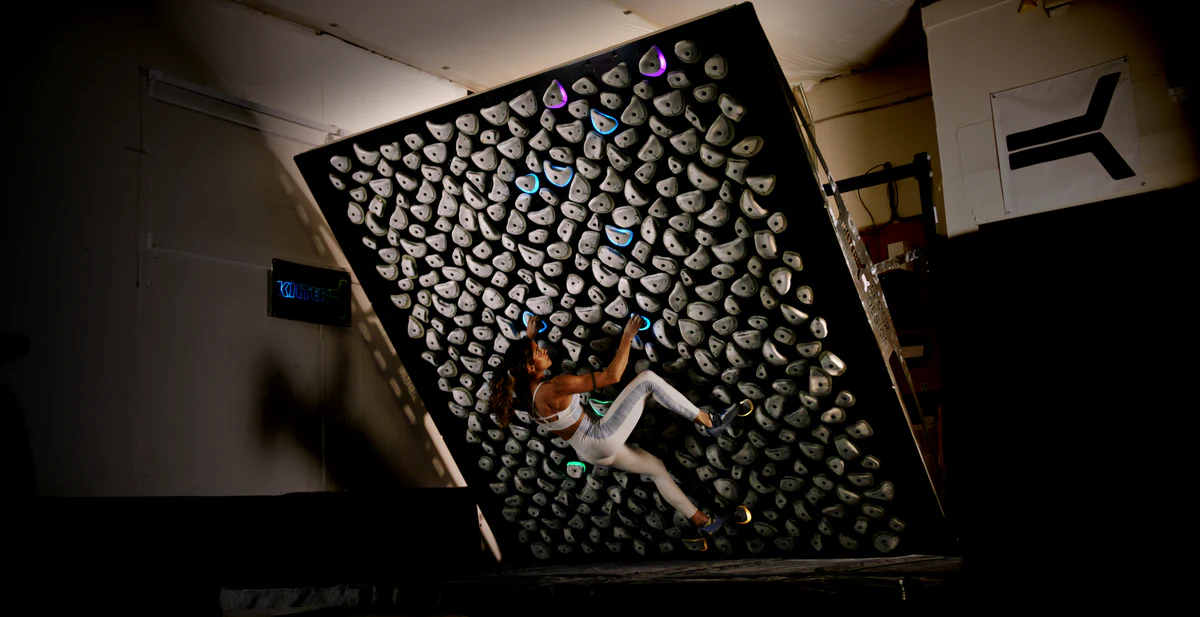
\includegraphics[width=0.9\linewidth]{kilter_example.png}
\caption{Fizyczna ściana Kilter Board z systemem chwytów podświetlanych LED.}
\label{fig:kilter-physical}
\end{figure}

\subsection{Opis problemu i sformułowanie zadania}
\label{sec:problem}

Projekt dotyczy opracowania warunkowego modelu generatywnego, którego zadaniem jest synteza sekwencji chwytów (tokenów trasy) dla systemu Kilter Board. Problem został sformalizowany jako generacja sekwencji dyskretnej (sekwencja tokenów ze skończonego słownika $\mathcal{V}$) z krótkiego kontekstu warunkującego:
\begin{itemize}[leftmargin=1.5em]
    \item identyfikatora układu panelu (\texttt{layout\_id}) --- jeden z dostępnych wariantów geometrii ściany,
    \item identyfikatora trudności (\texttt{grade\_id}) --- ocena V/Font (np.\ \texttt{6a/V3}).
\end{itemize}
Każda próbka ucząca ma postać:
\begin{equation}
\texttt{source} = [\texttt{layout\_id}, \texttt{grade\_id}], \quad
\texttt{target} = [t_1, t_2, \dots, t_n],
\end{equation}
gdzie $t_i \in \mathcal{V}$ to $i$-ty token sekwencji trasy (identyfikator chwytu lub rola), a $n$ to liczba kroków w trasie. Wektor \texttt{source} określa warunek generacji, a \texttt{target} stanowi wzorzec sekwencji pozycji chwytów.

\subsection{Charakterystyka zbioru danych}
\label{sec:dataset}

Wykorzystano publicznie dostępny zbiór tras Kilter Board \citep{kilterdataset}, przefiltrowany według następujących kryteriów:
\begin{itemize}[leftmargin=1.5em]
    \item minimalna liczba pierwszych przejść (\textit{ascensionists}): $\ge 5$,
    \item układ: \textit{Kilter Board Original} oraz \textit{Kilter Board Homewall},
    \item średnia ocena jakości (\textit{quality rating}): $> 2{,}6$,
    \item liczba klatek (\textit{frames count}): 1.
\end{itemize}
W rezultacie korpus zawiera \(N = 222\,624\) tras po wstępnym przetwarzaniu. Dla każdej próbki przygotowano słownik tokenów (\texttt{token\_to\_id}, \texttt{id\_to\_token}) o stałym rozmiarze, w którym wyróżniono trzy klasy tokenów:
\begin{itemize}[leftmargin=1.5em]
    \item \textbf{tokeny pozycji chwytów} (np.\ \texttt{p123}) --- numery otworów panelu,
    \item \textbf{tokeny ról} chwytów (start, top, hold, foot),
    \item \textbf{tokeny specjalne}: \texttt{<PAD>}, \texttt{<SOS>}, \texttt{<EOS>} (sekcja~\ref{sec:special-tokens}).
\end{itemize}

\begin{figure}[H]
\centering
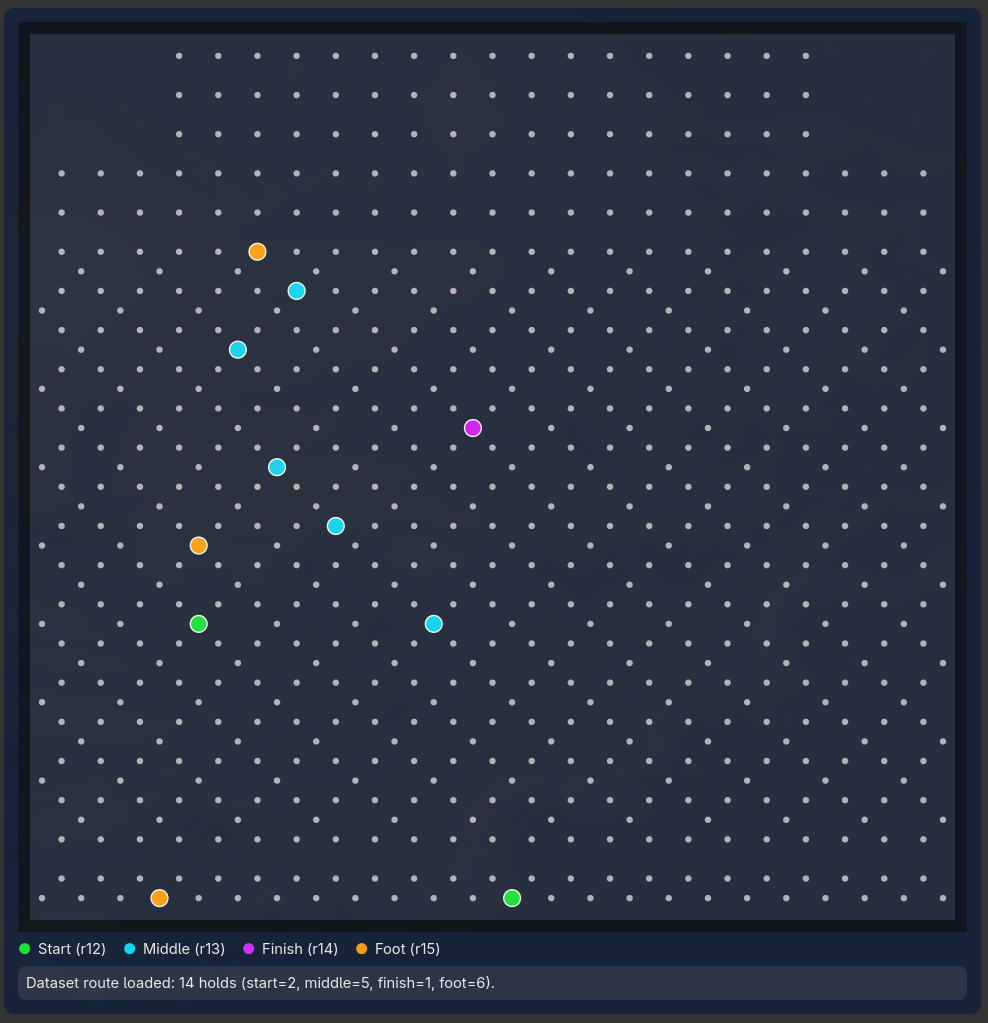
\includegraphics[width=0.9\linewidth]{loaded_route.png}
\caption{Przykładowa trasa z korpusu treningowego, zrenderowana w autorskim GUI.}
\label{fig:gui-example}
\end{figure}

\begin{figure}[H]
\centering
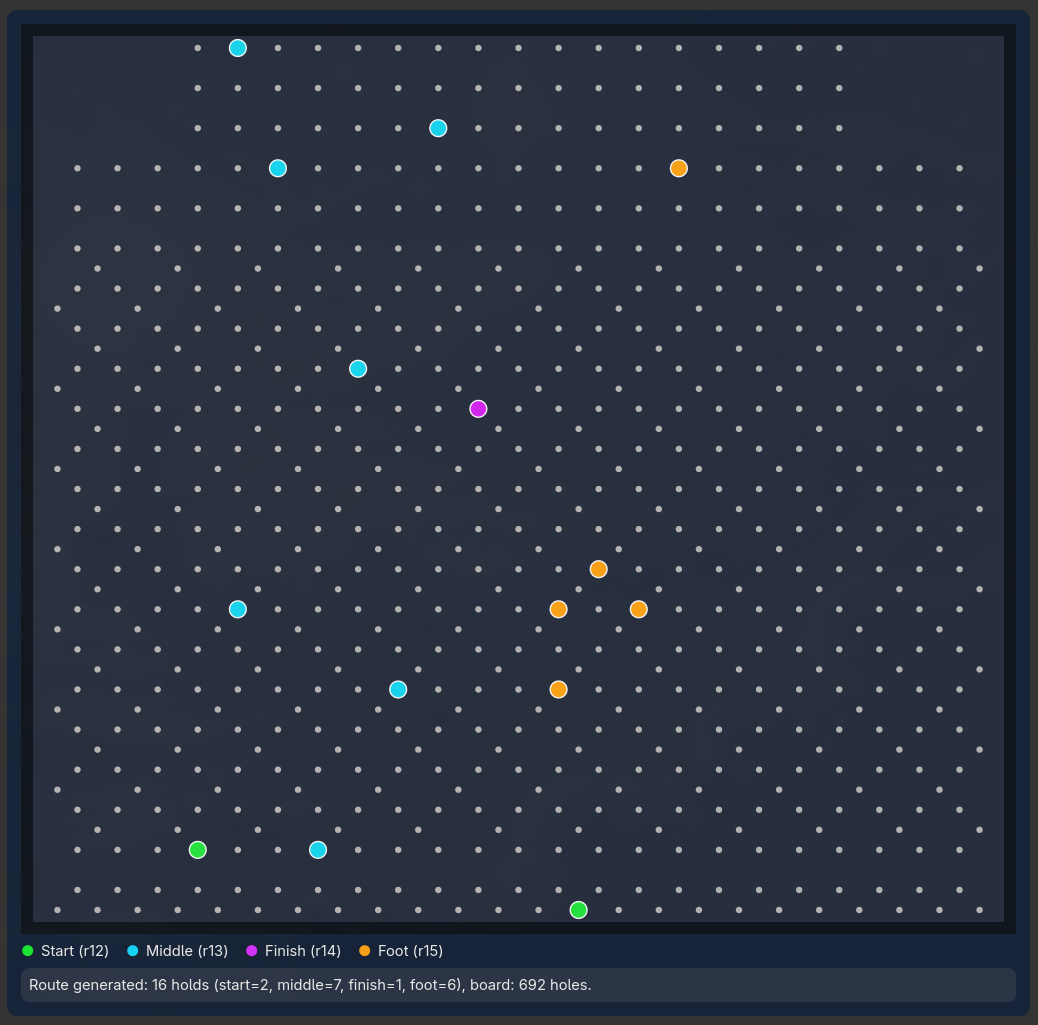
\includegraphics[width=0.9\linewidth]{generated_route.png}
\caption{Trasa wygenerowana przez model dla zadanej pary warunkującej.}
\label{fig:gui-generated}
\end{figure}

\subsection{Warstwy funkcjonalne projektu}

Realizacja projektu składa się z trzech warstw funkcjonalnych:
\begin{itemize}[leftmargin=1.5em]
    \item \textbf{warstwa danych} --- wczytanie korpusu tras, mapowanie tokenów oraz podział trening/walidacja,
    \item \textbf{warstwa modelu} --- sieć neuronowa typu warunkowy dekoder autoregresyjny (rozdz.~\ref{sec:architecture}),
    \item \textbf{warstwa inferencji} --- generacja tras z kontrolą losowości i przetwarzanie wyników do postaci użytecznej dla integracji z dowolnym interfejsem użytkownika.
\end{itemize}

\subsection{Struktura projektu}
\label{sec:project-structure}

Implementacja jest podzielona na trzy moduły, których krótki opis poniżej pozwala dalej w raporcie odwoływać się do nich \emph{nazwami funkcjonalnymi} (np.\ ,,moduł treningowy'', ,,skrypt scenariuszy'') zamiast bezpośrednio do ścieżek plików:
\begin{itemize}[leftmargin=1.5em]
    \item \textbf{moduł sieci} (katalog \texttt{kilter\_dl/}) --- jądro deep-learningowe projektu:
    \begin{itemize}[leftmargin=1.5em]
        \item \emph{definicja modelu} --- klasa \texttt{KilterRouteGenerator}, embeddingi warunkowe, dekoder GRU oraz głowa wyjściowa (rozdz.~\ref{sec:architecture}),
        \item \emph{moduł treningowy} --- wczytanie danych, grupowanie próbek w batche (funkcja \texttt{collate\_batch}), pętla uczenia AdamW, zapis checkpointów i metryk epokowych,
        \item \emph{moduł inferencji} --- generacja autoregresyjna z parametrami $\tau, k, p, \rho$ (rozdz.~\ref{sec:decoding}),
        \item \emph{skrypt scenariuszy eksperymentalnych} --- uruchamia 11 wariantów grupy A (uczenie) i 14 wariantów grupy B (generacja); wyniki tabelaryzowane w rozdz.~\ref{sec:experiments},
        \item \emph{katalog logów eksperymentów} (\texttt{logs/exp\_A*/}) --- metryki epokowe oraz podsumowanie konfiguracji każdego przebiegu uczenia,
        \item \emph{katalog checkpointów} (\texttt{checkpoints/}) --- najlepsze wagi modelu na walidacji, w tym \emph{checkpoint bazowy} (\texttt{exp\_A0\_baseline.pt}) używany do wszystkich scenariuszy generacji,
        \item \emph{katalog próbek} (\texttt{samples/exp\_B*/}) --- wygenerowane trasy w formacie JSON.
    \end{itemize}
    \item \textbf{moduł raportowy} (katalog \texttt{kilter\_report/}) --- niezależna biblioteka Pythona do produkcji wykresów raportu z surowych logów i plików próbek:
    \begin{itemize}[leftmargin=1.5em]
        \item \emph{generator wykresów} --- renderuje wszystkie figury sekcji~\ref{sec:experiments} do plików PDF (wektorowo),
        \item \emph{skrypt uruchomieniowy} --- pojedynczy punkt wejścia do procesu generowania rysunków.
    \end{itemize}
    \item \textbf{moduł raportu} (katalog \texttt{report/}) --- źródła niniejszego dokumentu LaTeX (\texttt{raport.tex}, \texttt{raport.bib}) wraz z podkatalogiem \texttt{figures/} na wyrenderowane wykresy.
\end{itemize}
W dalszej części raportu odniesienia do kodu i artefaktów eksperymentów przyjmują postać krótkich nazw funkcjonalnych zdefiniowanych powyżej.

\subsection{Zakres implementacyjny projektu}

Poniższy fragment kodu ilustruje główne etapy procesu uczenia:

\begin{lstlisting}[language=Python,caption={Szkielet procedury treningowej --- moduł treningowy.}]
token_to_id = load_json(args.token_map)
pad_id = token_to_id["<PAD>"]
sos_id = token_to_id["<SOS>"]
eos_id = token_to_id["<EOS>"]

samples_raw = load_json(args.dataset)
layout_to_idx, grade_to_idx = build_layout_grade_ids(samples_raw)
samples = [remap_source(s, layout_to_idx, grade_to_idx) for s in samples_raw]

model = KilterRouteGenerator(...).to(device)
optimizer = torch.optim.AdamW(model.parameters(), lr=args.lr)
\end{lstlisting}

Powyższy kod formalizuje trzy kluczowe decyzje projektowe: (i) jawne użycie tokenów specjalnych \texttt{<PAD>}, \texttt{<SOS>}, \texttt{<EOS>} (sekcja~\ref{sec:special-tokens}), (ii) separację przestrzeni tokenów wejściowych warunku od indeksacji używanej przez embeddingi warunkowe, (iii) optymalizację parametryczną metodą AdamW \citep{loshchilov2019adamw}.

Dla konfiguracji eksperymentalnej oznaczonej jako \texttt{report\_full} zastosowano pełny zbiór danych:
\begin{itemize}[leftmargin=1.5em]
    \item liczba próbek całkowita: 222\,624,
    \item zbiór treningowy: 220\,397,
    \item zbiór walidacyjny: 2\,227,
    \item najlepszy wynik walidacyjny: \texttt{best\_val\_nll = 0.8576}.
\end{itemize}
Powyższe wartości wskazują, że model osiąga użyteczny poziom dopasowania do rozkładu danych treningowych przy zachowaniu zadowalającej jakości na walidacji. Szersza dyskusja schematu doboru zbioru walidacyjnego znajduje się w sekcji~\ref{sec:validation}.

\section{Wstęp teoretyczny}

\subsection{Sieci neuronowe --- pojęcia podstawowe}
\label{sec:nn-intro}

Zanim przejdziemy do specyficznych zagadnień modelowania sekwencji, warto przypomnieć ogólny schemat działania sieci neuronowej. \emph{Sieć neuronowa} to parametryczna funkcja $f_\theta: \mathbb{R}^{d_{\text{in}}} \to \mathbb{R}^{d_{\text{out}}}$ zbudowana ze złożonych transformacji afinicznych przeplatanych nieliniowościami:
\begin{equation}
    h^{(\ell)} = \phi^{(\ell)}\!\left(W^{(\ell)} h^{(\ell-1)} + b^{(\ell)}\right),\quad \ell = 1,\dots,L,
\end{equation}
gdzie:
\begin{itemize}[leftmargin=1.5em]
    \item $h^{(0)} = x \in \mathbb{R}^{d_{\text{in}}}$ --- wejście,
    \item $W^{(\ell)}, b^{(\ell)}$ --- wagi i bias warstwy $\ell$,
    \item $\phi^{(\ell)}$ --- funkcja aktywacji (np.\ $\tanh$, ReLU, sigmoidalna),
    \item $h^{(L)}$ --- wyjście modelu.
\end{itemize}
Kluczową cechą sieci jest \emph{uczenie} parametrów $\theta = \{W^{(\ell)}, b^{(\ell)}\}$ poprzez minimalizację funkcji kosztu $\mathcal{L}(\theta)$ metodą gradientu wstecznego (\emph{backpropagation}) \citep{rumelhart1986backprop}. Schemat poglądowy gęstej sieci feedforward przedstawia rysunek~\ref{fig:nn-mlp}.

\begin{figure}[H]
\centering
\begin{tikzpicture}[
    >={Latex[length=2mm]},
    every neuron/.style={circle, draw, minimum size=7mm, inner sep=0pt, font=\footnotesize},
    in neuron/.style={every neuron, fill=blue!12},
    hid neuron/.style={every neuron, fill=green!12},
    out neuron/.style={every neuron, fill=orange!15},
    bias neuron/.style={every neuron, fill=gray!12, dashed, font=\scriptsize},
    layer label/.style={font=\small\bfseries, align=center}
]
    \foreach \i/\lab in {1/x_1, 2/x_2, 3/x_3}
      \node[in neuron] (in-\i) at (0, -\i*1.0 + 0.6) {$\lab$};
    \node[layer label, above=4mm of in-1] {Wejście\\$x \in \mathbb{R}^{d_{\text{in}}}$};

    \foreach \i in {1,...,4}
      \node[hid neuron] (h1-\i) at (3.0, -\i*0.9 + 0.7) {};
    \node[layer label, above=4mm of h1-1] {Warstwa ukryta 1\\$h^{(1)} = \phi(W^{(1)} x + b^{(1)})$};

    \foreach \i in {1,...,4}
      \node[hid neuron] (h2-\i) at (7.5, -\i*0.9 + 0.7) {};
    \node[layer label, above=4mm of h2-1] {Warstwa ukryta 2\\$h^{(2)} = \phi(W^{(2)} h^{(1)} + b^{(2)})$};

    \foreach \i/\lab in {1/y_1, 2/y_2}
      \node[out neuron] (out-\i) at (11.0, -\i*0.9 - 0.4) {$\lab$};
    \node[layer label, above=4mm of out-1] {Wyjście\\$y = h^{(L)}$};

    \foreach \i in {1,...,3}
      \foreach \j in {1,...,4}
        \draw[->, gray!55, thin] (in-\i) -- (h1-\j);
    \foreach \i in {1,...,4}
      \foreach \j in {1,...,4}
        \draw[->, gray!55, thin] (h1-\i) -- (h2-\j);
    \foreach \i in {1,...,4}
      \foreach \j in {1,...,2}
        \draw[->, gray!55, thin] (h2-\i) -- (out-\j);
\end{tikzpicture}
\caption{Wektorowy schemat gęstej sieci neuronowej feedforward. Każdy węzeł reprezentuje jednostkę obliczeniową, każda krawędź --- wagę $W^{(\ell)}_{ij}$. Sygnał przepływa od wejścia $x$ przez kolejne warstwy ukryte $h^{(\ell)}$ aż do wyjścia $y$. Analogiczną zasadę przepływu wykorzystuje dekoder GRU zastosowany w projekcie (rys.~\ref{fig:net-arch}), z tą różnicą, że kolejne transformacje są rozwijane w czasie po krokach sekwencji, a parametry są współdzielone między krokami.}
\label{fig:nn-mlp}
\end{figure}

W projekcie wykorzystano specjalizowaną odmianę takiej sieci --- \emph{rekurencyjną sieć neuronową} (rozdz.~\ref{sec:rnn-gru}) --- w której kolejne transformacje powstają przez \emph{rozwinięcie w czasie}: ten sam zestaw wag jest aplikowany w każdym kroku sekwencji, a stan ukryty $h_t$ pełni rolę reprezentacji historii przenoszonej między krokami.

\subsection{Tokeny specjalne w modelach sekwencyjnych}
\label{sec:special-tokens}

Modele sekwencyjne typu encoder--decoder oraz dekodery autoregresyjne operują na słownikach tokenów $\mathcal{V}$ zawierających zarówno tokeny \emph{semantyczne} (reprezentujące element domeny, tu: chwyty), jak i tokeny \emph{sterujące}. W projekcie wprowadzono trzy tokeny specjalne pochodzące z klasycznego paradygmatu \textit{seq2seq} \citep{sutskever2014seq2seq}:

\begin{itemize}[leftmargin=1.5em]
    \item \texttt{<SOS>} (\textit{Start Of Sequence}) --- pierwszy element wejścia dekodera w fazie inferencji. Stanowi specjalny token, którego embedding jest wyuczonym sygnałem rozpoczęcia generacji. Bez \texttt{<SOS>} dekoder nie miałby zdefiniowanego warunku początkowego dla rozkładu autoregresyjnego $P(y_1\mid c)$.
    \item \texttt{<EOS>} (\textit{End Of Sequence}) --- token oznaczający zakończenie sekwencji. W uczeniu jest dołączany na koniec każdej trasy w \texttt{tgt\_out}, dzięki czemu model uczy się momentu zakończenia generacji. W inferencji wygenerowanie \texttt{<EOS>} powoduje zakończenie pętli dekodującej.
    \item \texttt{<PAD>} (\textit{Padding}) --- token zerowy używany do wyrównania długości sekwencji w batchu. Pozycje \texttt{<PAD>} są \emph{ignorowane} przez funkcję kosztu (\texttt{ignore\_index=pad\_id}); w przeciwnym razie model mógłby nadmiernie dopasować się do artefaktu dopełnienia sekwencji.
\end{itemize}

W kontekście algorytmów uczenia maszynowego seq-to-seq tokeny te pełnią kilka funkcji: (i) umożliwiają tworzenie macierzy batchy o stałej długości (PAD), (ii) determinują warunki brzegowe rozkładu (SOS startuje, EOS kończy), (iii) odsprzęgają reprezentację końca trasy od konkretnego chwytu --- bez \texttt{<EOS>} sieć musiałaby kodować koniec trasy poprzez kombinację pozycji ostatniego chwytu, co znacząco zaburzałoby semantykę słownika.

\subsection{Modelowanie sekwencji warunkowych}
\label{sec:cond-seq}

Rozwiązywany problem należy do klasy modelowania sekwencji warunkowych \citep{bengio2003nlm,sutskever2014seq2seq}. Celem jest aproksymacja rozkładu:
\begin{equation}
P(y_1, y_2, \dots, y_T \mid c),
\end{equation}
gdzie:
\begin{itemize}[leftmargin=1.5em]
    \item $y_t \in \mathcal{V}$ --- token w pozycji $t$ sekwencji wyjściowej,
    \item $T$ --- długość sekwencji,
    \item $c$ --- kontekst wejściowy (warunek); tutaj para $c = (\texttt{layout}, \texttt{grade})$,
    \item $\mathcal{V}$ --- skończony słownik tokenów.
\end{itemize}
Zgodnie z regułą łańcuchową prawdopodobieństwa łącznego:
\begin{equation}
P(y_{1:T}\mid c) = \prod_{t=1}^{T} P(y_t \mid y_{<t}, c),
\end{equation}
gdzie $y_{<t} \equiv (y_1,\dots,y_{t-1})$ to historia tokenów do kroku $t-1$. W praktyce model generuje kolejne tokeny trasy \emph{autoregresyjnie}, tzn.\ każdy następny token zależy od historii już wygenerowanych tokenów i warunku wejściowego.

\subsection{Formalizacja celu uczenia}
\label{sec:loss}

Niech $x$ oznacza kontekst $(\texttt{layout}, \texttt{grade})$, a $y_{1:T}$ sekwencję tokenów trasy. Uczenie przebiega przez minimalizację średniej wartości ujemnego logarytmu wiarygodności (\textit{Negative Log-Likelihood}, NLL):
\begin{equation}
\mathcal{L}_{NLL} = -\frac{1}{Z}\sum_{i=1}^{N}\sum_{t=1}^{T_i}
\log P_\theta\!\left(y_t^{(i)} \mid y_{<t}^{(i)}, x^{(i)}\right)\cdot \mathbb{1}\!\left[y_t^{(i)} \neq \texttt{<PAD>}\right],
\end{equation}
gdzie:
\begin{itemize}[leftmargin=1.5em]
    \item $N$ --- liczba próbek (par $(x^{(i)}, y^{(i)})$) w batchu/epoce,
    \item $T_i$ --- długość $i$-tej sekwencji docelowej (po dołączeniu \texttt{<EOS>}),
    \item $\theta$ --- parametry sieci (embeddingi, GRU, głowa wyjściowa),
    \item $P_\theta$ --- rozkład warunkowy modelowany przez sieć,
    \item $\mathbb{1}[\cdot]$ --- funkcja wskaźnikowa (maska pozycji niebędących \texttt{<PAD>}),
    \item $Z = \sum_i \sum_t \mathbb{1}\!\left[y_t^{(i)} \neq \texttt{<PAD>}\right]$ --- liczba \emph{rzeczywistych} tokenów (normalizacja).
\end{itemize}
Pominięcie pozycji \texttt{<PAD>} oznacza, że model jest trenowany wyłącznie na rzeczywistych pozycjach sekwencji, co eliminuje wpływ technicznego dopełnienia batchy i zapewnia, że gradient odpowiada rzeczywistej skali zadania.

\subsection{Rekurencyjne sieci neuronowe (RNN, LSTM, GRU)}
\label{sec:rnn-gru}

\paragraph{Klasyczne RNN.}
Rekurencyjne sieci neuronowe (\textit{Recurrent Neural Networks}) \citep{goodfellow2016dl} przetwarzają sekwencje krok po kroku, utrzymując \emph{stan ukryty} $h_t \in \mathbb{R}^{h}$, który podsumowuje całą historię:
\begin{equation}
h_t = \tanh\!\left(W_{xh}\, x_t + W_{hh}\, h_{t-1} + b_h \right),
\end{equation}
gdzie:
\begin{itemize}[leftmargin=1.5em]
    \item $x_t \in \mathbb{R}^{d_e}$ --- wejście (embedding tokenu) w kroku $t$,
    \item $W_{xh} \in \mathbb{R}^{h \times d_e}$, $W_{hh} \in \mathbb{R}^{h \times h}$ --- macierze wag,
    \item $b_h \in \mathbb{R}^{h}$ --- bias.
\end{itemize}
Klasyczne RNN cierpią jednak na problem \emph{zanikającego/eksplodującego gradientu} \citep{pascanu2013difficulty}: powtarzane mnożenie przez $W_{hh}$ w propagacji wstecznej w czasie powoduje wykładnicze tłumienie lub eksplozję gradientu po kilkudziesięciu krokach. W praktyce uniemożliwia to uczenie zależności długodystansowych.

\paragraph{LSTM.}
Architektura \textit{Long Short-Term Memory} \citep{hochreiter1997lstm} rozwiązuje problem zanikania gradientu, wprowadzając trzy bramki (\emph{input}, \emph{forget}, \emph{output}) i oddzielny \emph{stan komórki} $c_t$:
\begin{equation}
\begin{aligned}
i_t &= \sigma(W_i x_t + U_i h_{t-1} + b_i), \\
f_t &= \sigma(W_f x_t + U_f h_{t-1} + b_f), \\
o_t &= \sigma(W_o x_t + U_o h_{t-1} + b_o), \\
\tilde c_t &= \tanh(W_c x_t + U_c h_{t-1} + b_c), \\
c_t &= f_t \odot c_{t-1} + i_t \odot \tilde c_t, \\
h_t &= o_t \odot \tanh(c_t),
\end{aligned}
\end{equation}
gdzie:
\begin{itemize}[leftmargin=1.5em]
    \item $\sigma(\cdot)$ --- funkcja sigmoidalna,
    \item $\odot$ --- iloczyn Hadamarda (po współrzędnych),
    \item $i_t, f_t, o_t \in [0,1]^h$ --- wektory bramek wejścia, zapominania i wyjścia,
    \item $\tilde c_t \in \mathbb{R}^h$ --- kandydat na nowy stan komórki,
    \item $c_t, h_t$ --- stan komórki i ukryty w kroku $t$.
\end{itemize}
LSTM charakteryzuje się wysoką skutecznością, jednak wykorzystuje cztery zestawy wag i osobny stan komórki, co zwiększa rozmiar modelu i koszt obliczeń.

\paragraph{GRU.}
\textit{Gated Recurrent Unit} \citep{cho2014gru} jest uproszczeniem LSTM. Posiada dwie bramki: \emph{reset} ($r_t$) oraz \emph{update} ($z_t$), a stan komórki został zlany ze stanem ukrytym:
\begin{equation}
\begin{aligned}
z_t &= \sigma(W_z x_t + U_z h_{t-1} + b_z), \\
r_t &= \sigma(W_r x_t + U_r h_{t-1} + b_r), \\
\tilde h_t &= \tanh\!\left(W_h x_t + U_h (r_t \odot h_{t-1}) + b_h \right), \\
h_t &= (1 - z_t) \odot h_{t-1} + z_t \odot \tilde h_t,
\end{aligned}
\end{equation}
gdzie:
\begin{itemize}[leftmargin=1.5em]
    \item $z_t \in [0,1]^h$ --- bramka update; steruje proporcją mieszania starego stanu i nowego kandydata,
    \item $r_t \in [0,1]^h$ --- bramka reset; pozwala selektywnie ,,zapomnieć'' poprzedni stan przy obliczaniu kandydata $\tilde h_t$,
    \item $W_*, U_*$ --- macierze wagowe odpowiednich bramek.
\end{itemize}

\paragraph{Dlaczego GRU dla zadania Kilter?}
\citet{chung2014empirical} wykazali empirycznie, że dla sekwencji umiarkowanej długości GRU osiąga jakość porównywalną z LSTM przy mniejszej liczbie parametrów. W kontekście projektu Kilter:
\begin{enumerate}[leftmargin=1.5em]
    \item Sekwencje tokenów trasy są \emph{krótkie} (zwykle $T < 100$). Pełna pojemność bramki forget LSTM nie jest niezbędna.
    \item Mniejsza liczba parametrów (3 macierze na bramkę zamiast 4) zmniejsza ryzyko przeuczenia.
    \item Mniejszy koszt obliczeniowy --- około $25\%$ szybsze trenowanie na batchach przy tej samej liczbie warstw.
    \item Brak osobnego stanu komórki upraszcza implementację \emph{warunkowania} przez inicjalizację stanu początkowego --- wystarczy jeden wektor projekcji.
    \item W przeciwieństwie do architektur transformatorowych GRU dobrze sprawdza się przy małej liczbie warstw i bardzo krótkim kontekście warunkującym (dwa tokeny źródłowe), gdzie self-attention nie miałby istotnej przewagi indukcyjnej.
\end{enumerate}

\paragraph{Warunkowanie przez stan początkowy.}
W warstwie koncepcyjnej zastosowano architekturę \emph{conditional decoder}: kontekst $x$ nie jest dołączany do każdego kroku wejściowego, lecz kodowany do stanu początkowego dekodera $h_0$. Dzięki temu warunek oddziałuje globalnie na całą generowaną sekwencję, a wejścia dekodera (embeddingi tokenów) niosą informację wyłącznie o historii sekwencji.

\subsection{Uczenie przez teacher forcing i funkcja kosztu}

W treningu zastosowano schemat \textit{teacher forcing} \citep{williams1989tf}: na wejście dekodera w kroku $t$ podawany jest \emph{prawidłowy} token $y_{t-1}$ (z danych uczących), a nie token przewidziany przez model. Stabilizuje to uczenie i przyspiesza zbieżność, szczególnie w początkowych epokach, gdy rozkład modelu jest jeszcze prawie jednorodny.

Jako kryterium optymalizacji wykorzystano entropię krzyżową na poziomie tokenów (NLL) z ignorowaniem pozycji dopełnienia (\texttt{<PAD>}). Minimalizacja NLL odpowiada maksymalizacji wiarygodności sekwencji obserwowanych w danych.

\subsection{Dekodowanie probabilistyczne i wpływ parametrów generacji}
\label{sec:decoding}

W trakcie inferencji rozkład warunkowy $P_\theta(y_t \mid y_{<t}, x)$ służy do iteracyjnego losowania (lub maksymalizacji) kolejnych tokenów. Czysta strategia zachłanna (\textit{greedy}) wybiera token o największym prawdopodobieństwie:
\begin{equation}
y_t^{(\text{greedy})} = \arg\max_{y \in \mathcal{V}} P_\theta(y \mid y_{<t}, x),
\end{equation}
ale prowadzi do \emph{degeneracji tekstu} \citep{holtzman2020nucleus}: powtarzających się bloków i niskiej różnorodności. W projekcie zastosowano sterowane próbkowanie z czterema parametrami; ich znaczenie i wpływ na wynik opisano poniżej.

\paragraph{Temperatura $\tau$.}
Logity $z = (z_1,\dots,z_{|\mathcal{V}|}) \in \mathbb{R}^{|\mathcal{V}|}$ są skalowane przed normalizacją softmaksem:
\begin{equation}
\tilde P_\theta(y = v_i) = \frac{\exp(z_i / \tau)}{\sum_{j=1}^{|\mathcal{V}|} \exp(z_j / \tau)},
\end{equation}
gdzie:
\begin{itemize}[leftmargin=1.5em]
    \item $\tau > 0$ --- parametr temperatury,
    \item $z_i$ --- logit (nieznormalizowany wynik) tokenu $v_i \in \mathcal{V}$.
\end{itemize}
Dla $\tau \to 0$ rozkład zbiega do deterministycznego \textit{argmax}; dla $\tau = 1$ używany jest natywny rozkład modelu; dla $\tau > 1$ rozkład się spłaszcza, zwiększając różnorodność kosztem precyzji.

\paragraph{Top-$k$ \citep{fan2018topk}.}
W kroku $t$ zachowywane jest $k$ tokenów o największych logitach, pozostałe otrzymują prawdopodobieństwo zerowe (logit ustawiany na $-\infty$):
\begin{equation}
\mathcal{V}_k = \mathrm{TopK}_k\!\left(z_1,\dots,z_{|\mathcal{V}|}\right), \quad
\tilde P_\theta(y) = 0 \text{ dla } y \notin \mathcal{V}_k.
\end{equation}
Parametr $k$ kontroluje twardy próg dopuszczalnych kandydatów; małe $k$ ogranicza różnorodność i eliminuje mało prawdopodobne wybory, ale zbyt małe może prowadzić do nadmiernej monotoniczności.

\paragraph{Top-$p$ (\textit{nucleus sampling}) \citep{holtzman2020nucleus}.}
Niech $\pi$ będzie permutacją indeksów malejąco po prawdopodobieństwie, a $\hat P$ rozkładem po softmaksie. Definiujemy najmniejszy zbiór $\mathcal{V}_p$:
\begin{equation}
\mathcal{V}_p = \left\{ v_{\pi(1)},\dots,v_{\pi(K)} \right\},\quad
K = \min \left\{ k : \sum_{j=1}^{k} \hat P\!\left(v_{\pi(j)}\right) \ge p \right\}.
\end{equation}
Tylko tokeny z $\mathcal{V}_p$ są kandydatami do wylosowania. W przeciwieństwie do top-$k$, top-$p$ adaptacyjnie dobiera rozmiar zbioru wyboru: w obszarach wysokiej koncentracji prawdopodobieństwa zbiór jest mały, natomiast w pozycjach o większej niepewności --- większy.

\paragraph{Repetition penalty $\rho \ge 1$.}
Niech $\mathcal{H}_t = \{y_1,\dots,y_{t-1}\}$ będzie zbiorem unikalnych tokenów już wygenerowanych. Dla $v \in \mathcal{H}_t$:
\begin{equation}
z'_v = \begin{cases} z_v / \rho & \text{jeżeli } z_v > 0, \\ z_v \cdot \rho & \text{jeżeli } z_v \le 0, \end{cases}
\end{equation}
co zmniejsza prawdopodobieństwo ponownego wylosowania już użytego tokenu. Im większe $\rho$, tym silniejsza redukcja prawdopodobieństwa powtórzeń.

\paragraph{Wpływ parametrów w praktyce.}
\begin{itemize}[leftmargin=1.5em]
    \item \emph{Zwiększenie $\tau$} $\Rightarrow$ trasy bardziej zróżnicowane, ale rośnie ryzyko nielogicznych przeskoków chwytów.
    \item \emph{Zmniejszenie $\tau$} $\Rightarrow$ trasy bardziej powtarzalne, bliższe ,,modalnej'' trasie z danych.
    \item \emph{Małe $k$ i małe $p$} $\Rightarrow$ wynik staje się bardziej deterministyczny, jakość pojedynczej próbki może wzrosnąć, ale generator jest bardziej podatny na lokalne pętle (przypadek Top-1).
    \item \emph{Duże $k$ / $p$ bliskie $1$} $\Rightarrow$ wynik bardziej różnorodny, ale podatny na błędy modelu w ogonie rozkładu.
    \item \emph{Wysokie $\rho$} $\Rightarrow$ ogranicza pętle, ale może wymuszać nieuzasadnione pomijanie chwytu, który naturalnie występuje wielokrotnie (np.\ chwyty pośrednie).
\end{itemize}
W konfiguracji projektowej przyjęto $\tau = 1{,}15$, $k = 40$, $p = 0{,}95$, $\rho = 1{,}1$, co empirycznie zapewnia akceptowalny kompromis pomiędzy różnorodnością a poprawnością.

\section{Realizacja sieci}

\subsection{Reprezentacja danych i przygotowanie batchy}

Dane wejściowe są zapisane jako listy identyfikatorów całkowitoliczbowych. Każda próbka zawiera:
\begin{itemize}[leftmargin=1.5em]
    \item \texttt{source}: dwa tokeny (\texttt{layout\_id}, \texttt{grade\_id}),
    \item \texttt{target}: sekwencję tokenów trasy.
\end{itemize}

W preprocessingu tworzona jest osobna indeksacja dla layoutów i poziomów trudności (\texttt{layout\_to\_idx}, \texttt{grade\_to\_idx}), co zapewnia zwarte zakresy indeksów dla embeddingów warunkowych.

Funkcja \texttt{collate\_batch} buduje dwa warianty sekwencji docelowej:
\begin{itemize}[leftmargin=1.5em]
    \item \texttt{tgt\_in} = $[\texttt{<SOS>}, t_1, \dots, t_n]$,
    \item \texttt{tgt\_out} = $[t_1, \dots, t_n, \texttt{<EOS>}]$,
\end{itemize}
następnie dopełnia obie macierze do maksymalnej długości w batchu tokenem \texttt{<PAD>}.

\begin{lstlisting}[language=Python,caption={Budowa par \texttt{tgt\_in}/\texttt{tgt\_out} (\texttt{collate\_batch}).}]
for t in targets:
    tgt_in = torch.cat([torch.tensor([sos_id]), t], dim=0)
    tgt_out = torch.cat([t, torch.tensor([eos_id])], dim=0)
    tgt_in_list.append(tgt_in)
    tgt_out_list.append(tgt_out)
\end{lstlisting}

Powyższa konstrukcja realizuje standardowe przesunięcie sekwencji o jeden krok (ang.\ \textit{next-token prediction}), co jest podstawą uczenia autoregresyjnego.

\subsection{Architektura modelu}
\label{sec:architecture}

Model \texttt{KilterRouteGenerator} składa się z trzech embeddingów:
\begin{itemize}[leftmargin=1.5em]
    \item embedding tokenów sekwencji $E_{\text{tok}} \in \mathbb{R}^{|\mathcal{V}|\times d_e}$,
    \item embedding layoutu $E_{\text{lay}} \in \mathbb{R}^{|\mathcal{L}|\times d_e}$,
    \item embedding grade $E_{\text{gr}} \in \mathbb{R}^{|\mathcal{G}|\times d_e}$,
\end{itemize}
gdzie:
\begin{itemize}[leftmargin=1.5em]
    \item $d_e$ --- wymiar embeddingu (w eksperymencie $d_e = 128$),
    \item $|\mathcal{L}|, |\mathcal{G}|$ --- rozmiary słowników layoutów i ocen trudności,
    \item $h$ --- wymiar stanu ukrytego GRU (w eksperymencie $h = 256$).
\end{itemize}
Embedding layoutu i grade są konkatenowane i projekcjonowane liniowo do przestrzeni stanu ukrytego przez warstwę \texttt{Linear+Tanh}. Otrzymany wektor pełni rolę stanu początkowego dekodera GRU i jest kopiowany na wszystkie warstwy rekurencyjne. W poprawionej wersji modelu ten sam kontekst jest również opcjonalnie dołączany do każdego kroku wejściowego dekodera (\texttt{condition\_every\_step}). Dzięki temu informacja o układzie panelu i trudności nie musi być przechowywana wyłącznie w stanie początkowym $h_0$, co ogranicza jej stopniowe zanikanie przy dłuższych generacjach.

Schematycznie działanie modelu prezentuje rysunek~\ref{fig:net-arch}.

\begin{figure}[H]
\centering
\begin{tikzpicture}[
    node distance=0.9cm and 1.3cm,
    box/.style={draw, rounded corners, minimum width=2.3cm, minimum height=0.75cm, align=center, font=\small},
    embed/.style={box, fill=blue!10},
    gru/.style={box, fill=green!10, minimum width=2.6cm},
    proj/.style={box, fill=orange!15},
    head/.style={box, fill=red!10},
    inp/.style={font=\small\itshape, align=center},
    >={Latex[length=2mm]}
]
    \node[inp] (layoutin) {layout\_id};
    \node[inp, right=2.3cm of layoutin] (gradein) {grade\_id};
    \node[inp, right=2.3cm of gradein] (tokin) {tgt\_in (z \texttt{<SOS>})};

    \node[embed, below=of layoutin] (Elay) {Embedding\\layoutu};
    \node[embed, below=of gradein] (Egr) {Embedding\\grade};
    \node[embed, below=of tokin] (Etok) {Embedding\\tokenów};

    \node[proj, below=of $(Elay)!0.5!(Egr)$] (cat) {Konkatenacja $[\cdot \,;\, \cdot]$};
    \node[proj, below=of cat] (proj) {Linear + Tanh\\\footnotesize($2d_e \to h$)};
    \node[proj, below=0.9cm of Etok] (fusion) {Fuzja wejścia\\\footnotesize($[E_{tok};E_{lay};E_{gr}]\to d_e$)};

    \node[gru, below=1.2cm of fusion] (gru) {GRU\\\footnotesize $L$ warstw, hidden=$h$};

    \node[head, below=of gru] (drop) {Dropout};
    \node[head, below=of drop] (head) {Linear\\\footnotesize($h \to |\mathcal{V}|$)};
    \node[inp, below=of head] (out) {logity\\$\to$ softmax};

    \draw[->] (layoutin) -- (Elay);
    \draw[->] (gradein) -- (Egr);
    \draw[->] (tokin) -- (Etok);
    \draw[->] (Elay) |- (cat);
    \draw[->] (Egr) |- (cat);
    \draw[->] (cat) -- (proj);
    \draw[->] (proj.east) -| node[pos=0.25, above, font=\footnotesize] {$h_0$} (gru.west);
    \draw[->] (Etok) -- (fusion);
    \draw[->, dashed] (cat.east) -| node[pos=0.25, above, font=\footnotesize] {$c$} (fusion.west);
    \draw[->] (fusion) -- (gru);
    \draw[->] (gru) -- (drop);
    \draw[->] (drop) -- (head);
    \draw[->] (head) -- (out);
\end{tikzpicture}
\caption{Architektura warunkowego dekodera GRU \texttt{KilterRouteGenerator}. Para $(\texttt{layout\_id}, \texttt{grade\_id})$ koduje stan początkowy $h_0$ oraz, w ulepszonym wariancie, jest dołączana do wejścia każdego kroku dekodera.}
\label{fig:net-arch}
\end{figure}

Sekwencja \texttt{tgt\_in} przechodzi przez dekoder GRU, po czym stosowany jest dropout i warstwa liniowa wyjściowa mapująca stan ukryty na logity po całym słowniku tokenów.

\begin{lstlisting}[language=Python,caption={Definicja modelu --- moduł architektury.}]
self.token_embedding = nn.Embedding(vocab_size, embed_dim)
self.layout_embedding = nn.Embedding(layout_vocab_size, embed_dim)
self.grade_embedding = nn.Embedding(grade_vocab_size, embed_dim)
self.context_proj = nn.Sequential(
    nn.Linear(embed_dim * 2, hidden_dim),
    nn.Tanh(),
)
self.input_fusion = nn.Sequential(
    nn.Linear(embed_dim * 3, embed_dim),
    nn.Tanh(),
)  # gdy condition_every_step=True
self.decoder = nn.GRU(input_size=embed_dim, hidden_size=hidden_dim,
                      num_layers=num_layers, batch_first=True)
self.head = nn.Linear(hidden_dim, vocab_size)
\end{lstlisting}

\begin{lstlisting}[language=Python,caption={Inicjalizacja stanu ukrytego z warunku --- moduł architektury.}]
layout_vec = self.layout_embedding(source[:, 0])
grade_vec = self.grade_embedding(source[:, 1])
context = torch.cat([layout_vec, grade_vec], dim=-1)
hidden0 = self.context_proj(context).unsqueeze(0)
return hidden0.repeat(self.decoder.num_layers, 1, 1)
\end{lstlisting}

\begin{lstlisting}[language=Python,caption={Fuzja kontekstu z tokenem wejściowym w każdym kroku dekodera.}]
token_vec = self.token_embedding(tgt_input)
context = self.context_embedding(source).unsqueeze(1)
context = context.expand(-1, tgt_input.shape[1], -1)
decoder_input = self.input_fusion(torch.cat([token_vec, context], dim=-1))
\end{lstlisting}

Interpretacyjnie: model uczy się funkcji $f:\mathbb{R}^{2d_e}\to\mathbb{R}^{h}$, która mapuje semantykę warunku (layout + grade) na punkt startowy dynamiki GRU. Ulepszona ścieżka \texttt{input\_fusion} dodatkowo uczy funkcji $g:\mathbb{R}^{3d_e}\to\mathbb{R}^{d_e}$, dzięki której każdy krok dekodera widzi zarówno historię tokenów, jak i jawny kontekst zadania. To zmniejsza ryzyko, że przy dłuższej sekwencji model zacznie generować trasę zgodną lokalnie z historią, ale słabiej dopasowaną do żądanej trudności lub layoutu.

\subsection{Procedura uczenia}

Uczenie realizowane jest optymalizatorem AdamW (sekcja~\ref{sec:adamw}) z clippingiem gradientu ($\|g\|_2 \le 1{,}0$) \citep{pascanu2013difficulty}. Dla każdej epoki obliczane są:
\begin{itemize}[leftmargin=1.5em]
    \item \texttt{train\_nll} --- strata na zbiorze treningowym,
    \item \texttt{val\_nll} --- strata walidacyjna,
    \item \texttt{val\_ppl} --- perplexity, $\exp(\texttt{val\_nll})$.
\end{itemize}
Najlepszy checkpoint jest zapisywany według kryterium minimalnego \texttt{val\_nll}, co ogranicza ryzyko nadmiernego dopasowania i pozwala zachować najbardziej użyteczną wersję modelu do generacji.

\begin{lstlisting}[language=Python,caption={Krok optymalizacji --- moduł treningowy.}]
logits = model(src, tgt_in)
loss = F.cross_entropy(
    logits.reshape(-1, logits.shape[-1]),
    tgt_out.reshape(-1),
    ignore_index=pad_id,
    reduction="sum",
)
token_count = (tgt_out != pad_id).sum().item()
(loss / max(1, token_count)).backward()
torch.nn.utils.clip_grad_norm_(model.parameters(), max_norm=1.0)
optimizer.step()
\end{lstlisting}

Istotnym szczegółem implementacyjnym jest normalizacja straty przez liczbę rzeczywistych tokenów (\texttt{token\_count}), a nie przez długość dopełnionego batcha. Dzięki temu estymator gradientu pozostaje porównywalny między batchami o różnych długościach sekwencji.

W badanym przebiegu (\texttt{report\_full}) wykorzystano m.in.\ parametry: \texttt{epochs=50}, \texttt{batch\_size=32}, \texttt{lr=0.001}, \texttt{embed\_dim=128}, \texttt{hidden\_dim=256}, \texttt{layers=3}, \texttt{dropout=0.15}, urządzenie \texttt{cuda}. Nowe treningi domyślnie włączają \texttt{condition\_every\_step=True}; starsze checkpointy pozostają kompatybilne, ponieważ parametr architektury jest zapisywany w konfiguracji modelu.

\subsection{Optymalizator AdamW}
\label{sec:adamw}

\paragraph{Geneza.}
AdamW \citep{loshchilov2019adamw} jest modyfikacją klasycznego optymalizatora Adam \citep{kingma2015adam}. Adam łączy momentum (pierwszy moment gradientu) z adaptacyjnym skalowaniem kroku per parametr (drugi moment). \citet{loshchilov2019adamw} zauważyli, że tradycyjna implementacja \emph{weight decay} w Adamie (dodanie członu $\lambda \theta$ do gradientu) splata regularyzację z momentum, co odbiega od formalnej definicji $L_2$-regularyzacji. AdamW \emph{rozprzęga} weight decay: jest on stosowany \emph{po} aktualizacji adaptacyjnej, bezpośrednio na wagach.

\paragraph{Algorytm.}
Niech $g_t \in \mathbb{R}^{|\theta|}$ będzie gradientem straty w kroku $t$.

\begin{algorithm}[H]
\caption{AdamW (Decoupled Weight Decay) --- \citep{loshchilov2019adamw}}
\label{alg:adamw}
\begin{algorithmic}[1]
\Require parametry $\theta_0$, krok uczenia $\eta$, współczynniki momentum $\beta_1, \beta_2 \in [0,1)$, weight decay $\lambda \ge 0$, stała numeryczna $\epsilon > 0$
\State $m_0 \gets 0$, $v_0 \gets 0$, $t \gets 0$
\While{nie osiągnięto kryterium stopu}
    \State $t \gets t + 1$
    \State $g_t \gets \nabla_\theta \mathcal{L}(\theta_{t-1})$ \Comment{gradient mini-batcha}
    \State $m_t \gets \beta_1\, m_{t-1} + (1 - \beta_1)\, g_t$ \Comment{pierwszy moment}
    \State $v_t \gets \beta_2\, v_{t-1} + (1 - \beta_2)\, g_t \odot g_t$ \Comment{drugi moment}
    \State $\hat m_t \gets m_t / (1 - \beta_1^t)$ \Comment{korekta obciążenia}
    \State $\hat v_t \gets v_t / (1 - \beta_2^t)$
    \State $\theta_t \gets \theta_{t-1} - \eta\!\left( \dfrac{\hat m_t}{\sqrt{\hat v_t} + \epsilon} + \lambda\, \theta_{t-1} \right)$ \Comment{aktualizacja + odsprzężony decay}
\EndWhile
\State \Return $\theta_t$
\end{algorithmic}
\end{algorithm}

Symbole:
\begin{itemize}[leftmargin=1.5em]
    \item $\theta_t$ --- parametry sieci w kroku $t$,
    \item $g_t$ --- gradient w kroku $t$,
    \item $m_t$ --- estymator wykładniczo ważonej średniej gradientów (momentum),
    \item $v_t$ --- estymator wykładniczo ważonej średniej kwadratów gradientu (skala),
    \item $\hat m_t, \hat v_t$ --- estymatory skorygowane o obciążenie (\emph{bias correction}),
    \item $\eta$ --- krok uczenia (\texttt{lr}); $\beta_1 = 0{,}9$, $\beta_2 = 0{,}999$ (wartości typowe),
    \item $\lambda$ --- współczynnik weight decay; $\epsilon \approx 10^{-8}$ --- stabilność numeryczna.
\end{itemize}

\paragraph{Zalety w kontekście projektu.}
\begin{itemize}[leftmargin=1.5em]
    \item \textbf{Adaptacyjny krok per parametr.} Embeddingi rzadko aktualizowanych tokenów (np.\ rzadkie layouty) otrzymują większą efektywną stopę uczenia niż gęsto używane macierze GRU.
    \item \textbf{Odsprzężony weight decay.} Zapewnia spójną regularyzację \emph{niezależną} od skali drugiego momentu --- empirycznie poprawia uogólnienie \citep{loshchilov2019adamw}.
    \item \textbf{Stabilność w mieszanych skalach.} W naszej architekturze współistnieją małe wagi głowy wyjściowej i większe wagi GRU; adaptacyjna skala zapobiega temu, by małe wagi były ,,zdominowane'' przez duże.
    \item \textbf{Odporność względem doboru learning rate.} W projekcie użyto $\eta = 10^{-3}$, co jest typowym i stabilnym wyborem dla AdamW na zadaniach językowych.
    \item \textbf{Małe wymagania pamięciowe} ($2|\theta|$ dodatkowych zmiennych --- $m, v$), znacznie mniejsze niż dla metod drugiego rzędu.
\end{itemize}

\subsection{Dobór zbioru walidacyjnego a walidacja krzyżowa}
\label{sec:validation}

W badaniach przyjęto \emph{trzymany} zbiór walidacyjny (\textit{held-out validation set}) o wielkości 1\% wszystkich próbek, czyli $|\mathcal{D}_{\text{val}}| = 2\,227$ tras, podczas gdy $|\mathcal{D}_{\text{train}}| = 220\,397$. Wybór ten został podjęty świadomie i zasługuje na komentarz w kontekście klasycznej walidacji krzyżowej.

\paragraph{Walidacja krzyżowa --- przypomnienie.}
W $k$-krotnej walidacji krzyżowej (\textit{$k$-fold cross-validation}) \citep{stone1974cv,kohavi1995cv} zbiór danych $\mathcal{D}$ dzielony jest na $k$ rozłącznych podzbiorów $\mathcal{D}^{(1)},\dots,\mathcal{D}^{(k)}$. Model trenowany jest $k$ razy --- za każdym razem na $\mathcal{D}\setminus\mathcal{D}^{(j)}$, ewaluowany na $\mathcal{D}^{(j)}$. Estymator błędu:
\begin{equation}
\widehat{\mathrm{CV}}_k = \frac{1}{k}\sum_{j=1}^{k} \mathcal{L}_{\text{val}}\!\left(\theta^{(j)};\, \mathcal{D}^{(j)}\right),
\end{equation}
gdzie:
\begin{itemize}[leftmargin=1.5em]
    \item $k$ --- liczba foldów (typowo $5$ lub $10$),
    \item $\theta^{(j)}$ --- parametry modelu wytrenowanego z pominięciem $j$-tego foldu,
    \item $\mathcal{L}_{\text{val}}$ --- funkcja kosztu na zbiorze walidacyjnym.
\end{itemize}
$\widehat{\mathrm{CV}}_k$ ma mniejszą wariancję niż pojedynczy split, ale wymaga $k$-krotnego trenowania modelu.

\paragraph{Dlaczego nie zastosowano $k$-fold CV?}
Decyzja o pojedynczym, ustalonym podziale danych została podjęta z następujących powodów:
\begin{enumerate}[leftmargin=1.5em]
    \item \textbf{Skala danych.} Korpus liczy $N = 222\,624$ tras. Przy tak dużym $N$ pojedyncza walidacja jest już dobrym estymatorem błędu generalizacji --- wariancja estymatora $\mathcal{L}_{\text{val}}$ malejąca jak $\mathcal{O}(1/|\mathcal{D}_{\text{val}}|)$ jest dostatecznie mała przy $|\mathcal{D}_{\text{val}}| > 2000$.
    \item \textbf{Koszt obliczeniowy.} Jedna pełna epoka trwa kilka minut na GPU; pełne 5-fold CV przy 50 epokach wymagałoby $5 \times 50 = 250$ przebiegów, co przy każdej zmianie konfiguracji byłoby nieproporcjonalne względem oczekiwanego zysku informacyjnego.
    \item \textbf{Cel: model, nie estymator.} Celem nie jest \emph{estymacja błędu generalizacji} z najwyższą możliwą precyzją, lecz \emph{wytrenowanie najlepszego dostępnego modelu} oraz użycie zbioru walidacyjnego jako kryterium wczesnego zatrzymania (\textit{early stopping}) i selekcji najlepszego checkpointu.
    \item \textbf{Brak rozbudowanego przeszukiwania hiperparametrów.} Hiperparametry zostały dobrane na podstawie literatury (rozmiary embeddingu, dropout, learning rate); $k$-fold CV jest szczególnie użyteczne przy szerokim \emph{grid search}, którego w niniejszej pracy nie prowadzono.
    \item \textbf{Wewnętrzna różnorodność.} Próbki są losowo tasowane (\texttt{random.shuffle(samples)} z ustalonym \texttt{seed=42}) przed splitem, co czyni zbiór walidacyjny reprezentatywnym względem rozkładu łącznego (warstwy trudności, layouty).
\end{enumerate}

\paragraph{Kiedy warto przejść na $k$-fold?}
W rozszerzonej fazie projektu (poza zakresem niniejszego raportu) wskazane byłoby:
\begin{itemize}[leftmargin=1.5em]
    \item \textbf{Stratified $k$-fold} po atrybucie \texttt{grade\_id} --- by zagwarantować, że rzadkie trudności są reprezentowane w każdym foldzie,
    \item \textbf{Grouped CV} po \texttt{layout\_id} --- gdy celem jest ocena uogólnienia modelu na \emph{niewidziane} układy panelu,
    \item \textbf{Repeated holdout} --- kompromis o niższym koszcie obliczeniowym niż pełna $k$-fold CV.
\end{itemize}
W obecnej fazie pojedynczy holdout 99\%/1\% pozostaje uzasadnionym kompromisem między precyzją szacunku, kosztem obliczeń i celami praktycznymi projektu.

\subsection{Generacja i postprocessing}

Po wczytaniu checkpointu model przyjmuje wejście $[\texttt{layout\_id}, \texttt{grade\_id}]$, mapuje je do indeksów treningowych i generuje sekwencję od tokenu \texttt{<SOS>} aż do \texttt{<EOS>} lub do osiągnięcia limitu długości. Wygenerowane tokeny specjalne są odfiltrowywane, a tokeny pozycji chwytów (np.\ \texttt{p123}) są konwertowane do listy numerów otworów panelu.

\begin{lstlisting}[language=Python,caption={Konfiguracja dekodowania --- moduł inferencji.}]
generated = model.generate(
    source=source,
    sos_id=ckpt["sos_id"],
    eos_id=ckpt["eos_id"],
    max_len=args.max_len,
    do_sample=not args.greedy,
    temperature=args.temperature,
    top_k=args.top_k,
    top_p=args.top_p,
    repetition_penalty=args.repetition_penalty,
)
\end{lstlisting}

Z punktu widzenia użytkowego mechanizm ten umożliwia sterowanie kompromisem pomiędzy deterministycznością a różnorodnością generacji, bez konieczności modyfikowania parametrów samej sieci (patrz sekcja~\ref{sec:decoding}). Tak przygotowany wynik może być bezpośrednio użyty przez kolejne moduły systemu (np.\ wizualizację/integrację), niezależnie od samego procesu uczenia.

\section{Wyniki eksperymentów}
\label{sec:experiments}

\subsection{Stanowisko eksperymentalne}
\label{sec:exp-setup}

W celu pomiaru wpływu pojedynczych hiperparametrów uczenia oraz parametrów dekodowania zrealizowano dwa zestawy scenariuszy zamknięte w skrypcie scenariuszy eksperymentalnych (rozdz.~\ref{sec:project-structure}):
\begin{itemize}[leftmargin=1.5em]
    \item \textbf{Grupa A (uczenie)} --- 11 niezależnych przebiegów treningowych, w których zmieniano po jednym hiperparametrze względem konfiguracji bazowej (\texttt{A0\_baseline}). Każdy przebieg zapisuje metryki epokowe oraz podsumowanie konfiguracji do osobnego katalogu wewnątrz katalogu logów eksperymentów.
    \item \textbf{Grupa B (generacja)} --- 14 wywołań inferencji z tym samym checkpointem bazowym (\texttt{exp\_A0\_baseline.pt}) i tym samym promptem $(\texttt{layout}=1272,\,\texttt{grade}=1240)$, czyli ,,12$\times$12 without kickboard Square'' / ,,6a+/V3''. Wyniki trafiają do katalogu próbek (po jednym pliku JSON na scenariusz).
\end{itemize}
Z uwagi na potrzebę szybkiego porównania trendów w grupie A użyto ograniczonego podzbioru (\texttt{MAX\_SAMPLES}=$20\,000$, \texttt{EPOCHS}=$5$, \texttt{VAL\_RATIO}=$0{,}05$, urządzenie CPU). Konfiguracja \texttt{report\_full} z sekcji~\ref{sec:problem} jest niezależna i służyła do walidacji jakościowej najlepszego modelu.

Wszystkie wykresy w niniejszej sekcji powstają bezpośrednio z surowych logów eksperymentów --- za ich produkcję odpowiada moduł raportowy (rozdz.~\ref{sec:project-structure}): generator wykresów renderuje rysunki do formatu PDF (wektorowo), a skrypt uruchomieniowy integruje cały proces w jedno polecenie.

\subsection{Wpływ parametrów uczenia}
\label{sec:exp-train}

Tabela~\ref{tab:exp-train} zestawia konfiguracje grupy A wraz z najlepszą wartością NLL na zbiorze walidacyjnym (\texttt{best\_val\_nll}), perplexity oraz średnim czasem epoki. Pełne krzywe uczenia w funkcji epoki przedstawiono na rysunkach~\ref{fig:train-lr}--\ref{fig:train-layers}, a zbiorcze rankingi --- na rysunkach~\ref{fig:summary-best} i \ref{fig:summary-time}.

\begin{table}[H]
\centering
\caption{Konfiguracje przebiegów treningowych (grupa A) oraz wyniki na walidacji. Wszystkie konfiguracje korzystają z optymalizatora AdamW z gradient clippingiem $\|g\|_2\le 1{,}0$.}
\label{tab:exp-train}
\small
\begin{tabular}{lccccccrrr}
\toprule
Eksperyment & lr & embed & hidden & L & dropout & bs & best val\_nll & val\_ppl & $\overline{t_{\text{ep}}}$ [s] \\
\midrule
A0\_baseline       & $10^{-3}$ & 128 & 256 & 3 & 0.15 & 64  & 1.752 & 5.76  & 41.9 \\
A1\_lr\_low        & $10^{-5}$ & 128 & 256 & 3 & 0.15 & 64  & 4.132 & 62.33 & 41.2 \\
A1\_lr\_high       & $10^{-2}$ & 128 & 256 & 3 & 0.15 & 64  & 2.228 & 9.28  & 44.8 \\
A2\_small\_model   & $10^{-3}$ & 64  & 64  & 1 & 0.15 & 64  & 2.240 & 9.39  & 7.8  \\
A2\_large\_model   & $10^{-3}$ & 256 & 512 & 4 & 0.15 & 64  & \textbf{1.395} & \textbf{4.03}  & 141.2 \\
A3\_dropout\_off   & $10^{-3}$ & 128 & 256 & 3 & 0.00 & 64  & 1.658 & 5.25  & 37.1 \\
A3\_dropout\_high  & $10^{-3}$ & 128 & 256 & 3 & 0.50 & 64  & 1.928 & 6.87  & 46.2 \\
A4\_batch\_small   & $10^{-3}$ & 128 & 256 & 3 & 0.15 & 16  & \textbf{1.337} & \textbf{3.81}  & 47.6 \\
A4\_batch\_large   & $10^{-3}$ & 128 & 256 & 3 & 0.15 & 256 & 2.192 & 8.95  & 55.7 \\
A5\_layers\_1      & $10^{-3}$ & 128 & 256 & 1 & 0.15 & 64  & 1.645 & 5.18  & 19.0 \\
A5\_layers\_5      & $10^{-3}$ & 128 & 256 & 5 & 0.15 & 64  & 1.902 & 6.70  & 66.6 \\
\bottomrule
\end{tabular}
\end{table}

\paragraph{Learning rate.}
Rysunek~\ref{fig:train-lr} wskazuje, że \texttt{lr}$=10^{-5}$ skutkuje niedouczeniem --- po 5 epokach \texttt{val\_nll}$\approx 4{,}13$, czyli model pozostaje zbliżony do początkowego rozkładu jednorodnego. Z drugiej strony \texttt{lr}$=10^{-2}$ wprowadza wyraźną niestabilność: w epokach 2--4 strata walidacyjna oscyluje (2.23 / 2.29 / 2.23), co obrazuje typowy efekt zbyt dużego kroku w AdamW. Wartość bazowa $10^{-3}$ prowadzi do najbardziej stabilnego przebiegu uczenia w tej grupie eksperymentów.

\begin{figure}[H]
\centering
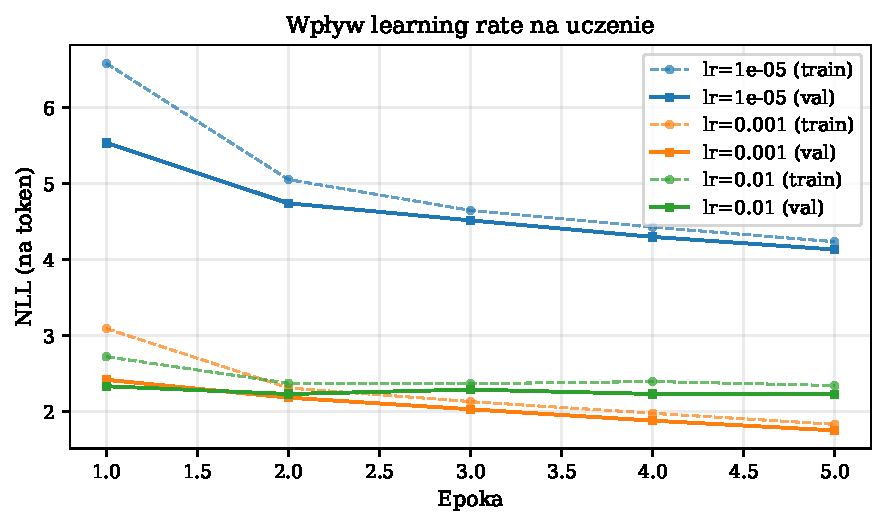
\includegraphics[width=0.95\linewidth]{fig_train_lr.pdf}
\caption{Krzywe \texttt{train\_nll} (linie przerywane) i \texttt{val\_nll} (linie ciągłe) dla różnych wartości \texttt{lr}.}
\label{fig:train-lr}
\end{figure}

\paragraph{Pojemność modelu.}
Wzrost wymiarów (\texttt{embed\_dim}, \texttt{hidden\_dim}) i głębokości (\texttt{layers}) przekłada się na lepsze dopasowanie. Konfiguracja \texttt{A2\_large} osiąga \texttt{val\_nll}$=1{,}395$ (najlepszy wynik wśród modeli porównywalnej długości treningu), ale przy ok.\ $3{,}4\times$ dłuższym czasie epoki. Model o mniejszej pojemności (\texttt{A2\_small}) jest $5\times$ szybszy, lecz krzywa uczenia wskazuje na ograniczenia jego pojemności reprezentacyjnej (rys.~\ref{fig:train-capacity}).

\begin{figure}[H]
\centering
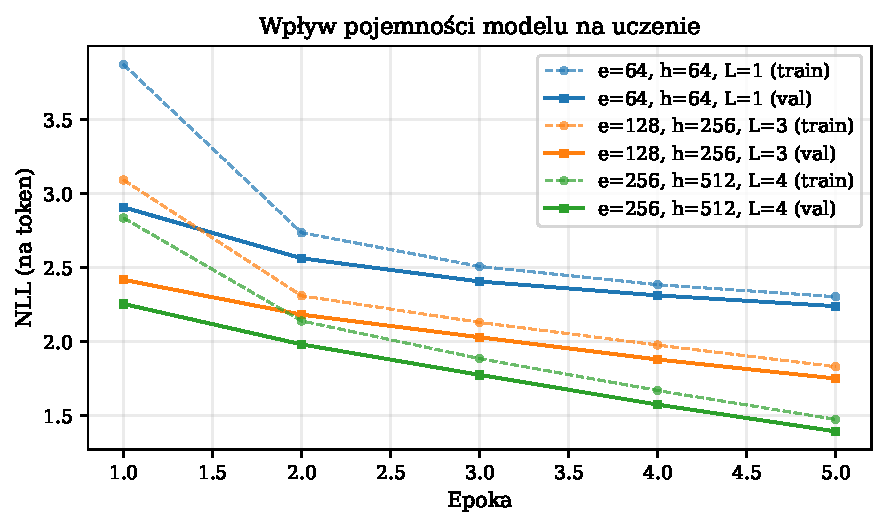
\includegraphics[width=0.95\linewidth]{fig_train_capacity.pdf}
\caption{Wpływ pojemności modelu (rozmiary embeddingu, stanu ukrytego i liczby warstw).}
\label{fig:train-capacity}
\end{figure}

\paragraph{Dropout.}
Na podzbiorze 20\,000 próbek włączenie \texttt{dropout=0{,}5} powoduje wyraźne pogorszenie (val\_nll $1{,}93$), a brak dropoutu skutkuje minimalnie lepszym wynikiem niż konfiguracja bazowa (1.66 vs 1.75). Sugeruje to, że przy ograniczonym budżecie danych i krótkim treningu dropout 0.5 nadmiernie tłumi sygnał. Dla pełnego korpusu 222 624 próbek umiarkowany dropout (0.15) jest natomiast uzasadniony --- chroni przed przeuczeniem przy dużej liczbie epok.

\begin{figure}[H]
\centering
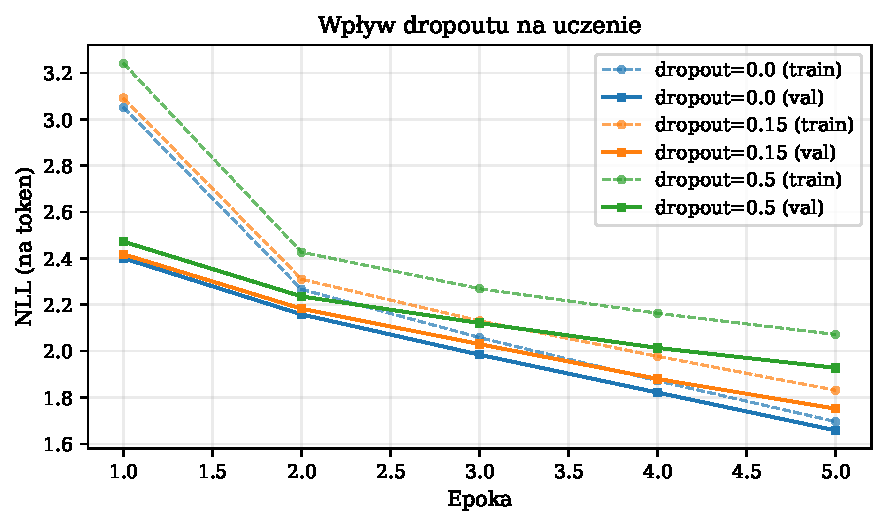
\includegraphics[width=0.95\linewidth]{fig_train_dropout.pdf}
\caption{Wpływ \texttt{dropout} na proces uczenia.}
\label{fig:train-dropout}
\end{figure}

\paragraph{Rozmiar batcha.}
Najbardziej korzystny wynik uzyskuje \texttt{A4\_batch\_small} (\texttt{bs}$=16$): \texttt{val\_nll}$=1{,}337$, co stanowi najlepszy wynik w grupie A poza modelem dużym. Wynika to z większej liczby kroków optymalizatora w epoce (1188 zamiast 297 przy \texttt{bs}$=64$ i 74 przy \texttt{bs}$=256$) oraz silniej stochastycznego gradientu, który pełni rolę regularyzatora \citep{loshchilov2019adamw}. Duży batch (\texttt{bs}$=256$) wyraźnie pogarsza wynik (val\_nll $2{,}19$).

\begin{figure}[H]
\centering
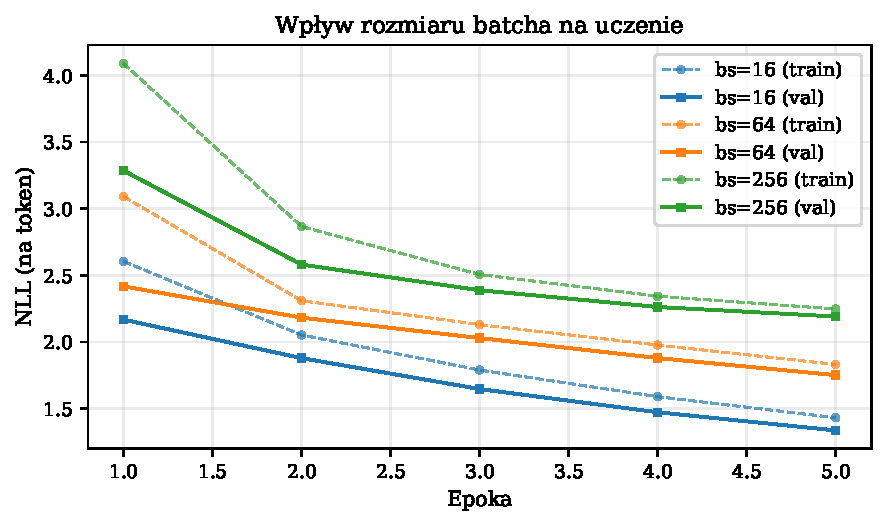
\includegraphics[width=0.95\linewidth]{fig_train_batch.pdf}
\caption{Wpływ rozmiaru batcha na zbieżność i jakość walidacji.}
\label{fig:train-batch}
\end{figure}

\paragraph{Liczba warstw GRU.}
Wbrew oczekiwaniom, \texttt{A5\_layers\_1} (jedna warstwa) osiąga \texttt{val\_nll}$=1{,}65$, czyli wynik lepszy niż baseline z trzema warstwami (1.75) oraz wariant pięciowarstwowy (1.90). Dla zadania o krótkich sekwencjach ($T<100$) i prostym kontekście warunkującym (2 tokeny) głęboki dekoder rekurencyjny nie poprawia wyników i wymaga więcej epok do efektywnego przekazania gradientu wstecznego. Zależność tę przedstawiają krzywe na rys.~\ref{fig:train-layers}.

\begin{figure}[H]
\centering
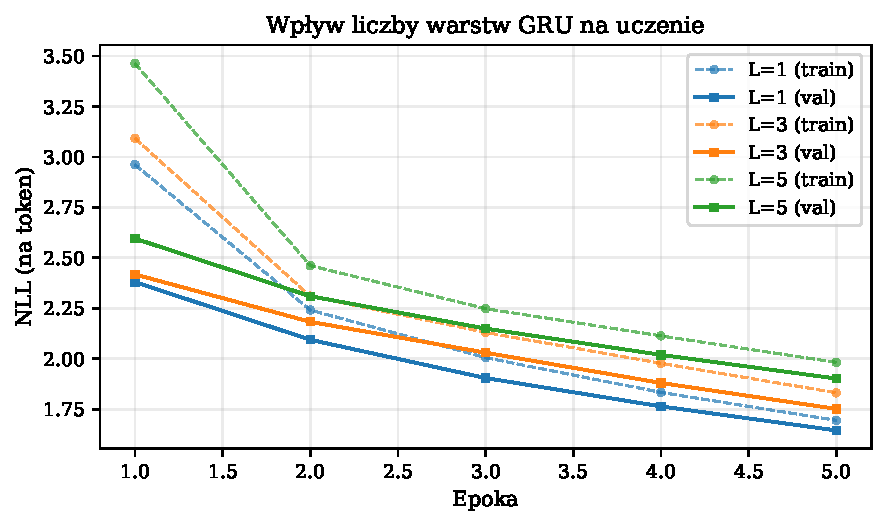
\includegraphics[width=0.95\linewidth]{fig_train_layers.pdf}
\caption{Wpływ liczby warstw GRU na proces uczenia.}
\label{fig:train-layers}
\end{figure}

\paragraph{Zbiorcze porównanie.}
Rysunki~\ref{fig:summary-best} i \ref{fig:summary-time} zestawiają najlepsze \texttt{val\_nll} oraz średni czas epoki dla wszystkich konfiguracji grupy A.

\begin{figure}[H]
\centering
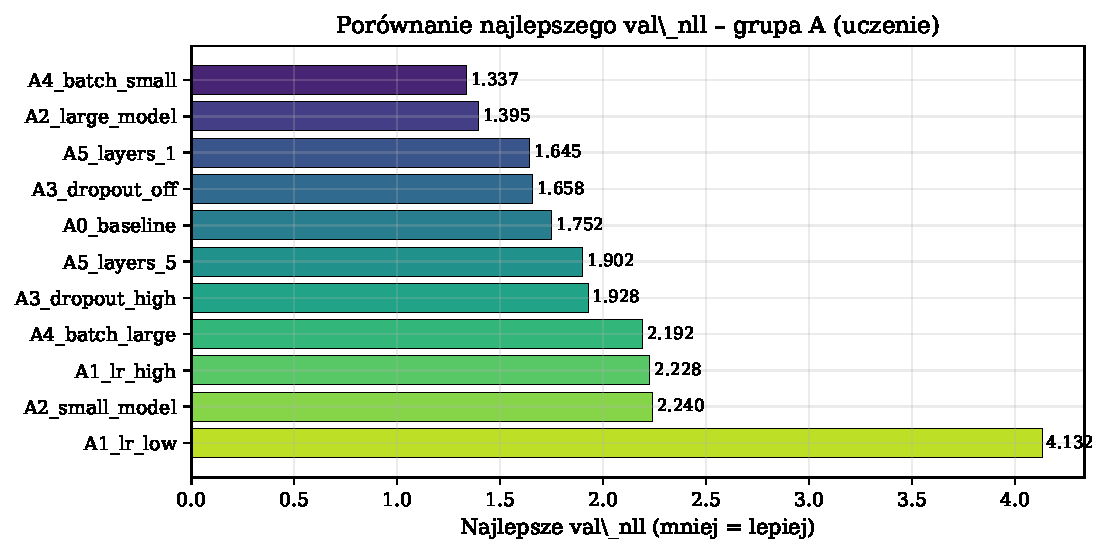
\includegraphics[width=0.95\linewidth]{fig_summary_best_val.pdf}
\caption{Ranking najlepszego \texttt{val\_nll} (mniej = lepiej) dla 11 konfiguracji uczenia.}
\label{fig:summary-best}
\end{figure}

\begin{figure}[H]
\centering
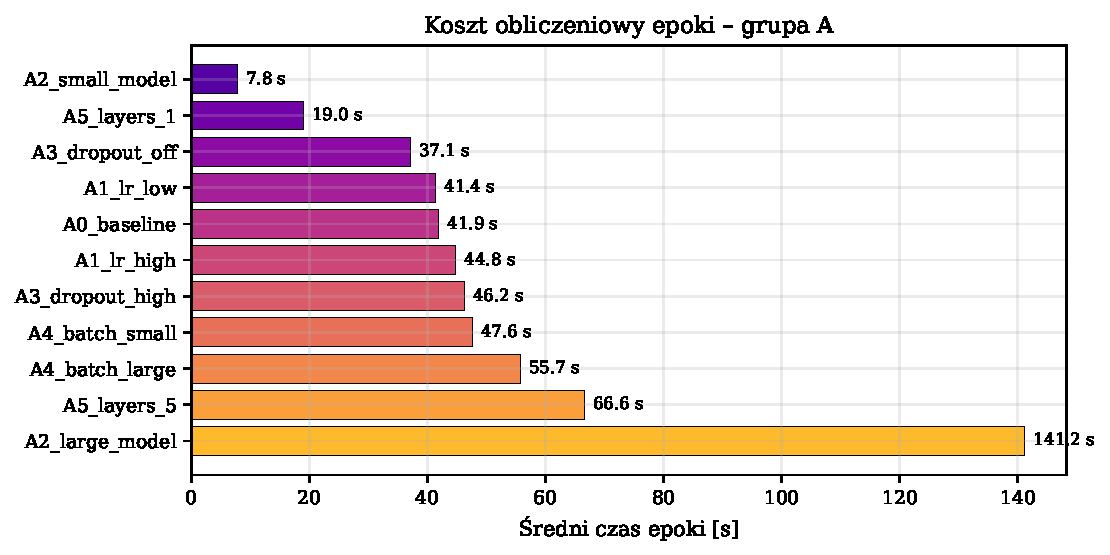
\includegraphics[width=0.95\linewidth]{fig_summary_epoch_time.pdf}
\caption{Średni czas epoki dla 11 konfiguracji uczenia (CPU).}
\label{fig:summary-time}
\end{figure}

\subsection{Wpływ parametrów generacji}
\label{sec:exp-gen}

W grupie B utrzymujemy stały checkpoint bazowy i zmieniamy parametry dekodowania. Tabela~\ref{tab:exp-gen} zestawia 14 scenariuszy oraz dwie podstawowe metryki na poziomie tokenów:
\begin{itemize}[leftmargin=1.5em]
    \item $n_h$ --- liczba chwytów (tokenów \texttt{p<id>}) wygenerowanych przed \texttt{<EOS>},
    \item $n_h^{\text{uniq}}/n_h$ --- udział unikalnych chwytów (rośnie, gdy model nie powtarza chwytów).
\end{itemize}

\begin{table}[H]
\centering
\caption{Konfiguracje dekodowania (grupa B) i statystyki wygenerowanej trasy dla promptu $(\texttt{layout}=1272,\,\texttt{grade}=1240)$. Pole ,,---'' oznacza, że dany parametr nie ma znaczenia w danym wariancie (greedy ignoruje wszystkie parametry losowe).}
\label{tab:exp-gen}
\small
\begin{tabular}{lccccrr}
\toprule
Eksperyment & $\tau$ & top-$k$ & top-$p$ & $\rho$ & $n_h$ & $n_h^{\text{uniq}}/n_h$ \\
\midrule
B0\_greedy        & ---  & ---  & ---  & ---  & 8  & 100\% \\
B1\_temp\_0.5     & 0.5  & 0    & 1.00 & 1.0  & 9  & 100\% \\
B1\_temp\_1.0     & 1.0  & 0    & 1.00 & 1.0  & 10 & 100\% \\
B1\_temp\_1.5     & 1.5  & 0    & 1.00 & 1.0  & 23 & 100\% \\
B2\_topk\_1       & 1.0  & 1    & 1.00 & 1.0  & 8  & 100\% \\
B2\_topk\_5       & 1.0  & 5    & 1.00 & 1.0  & 7  & 100\% \\
B2\_topk\_40      & 1.0  & 40   & 1.00 & 1.0  & 11 & 100\% \\
B3\_topp\_0.5     & 1.0  & 0    & 0.50 & 1.0  & 8  & 100\% \\
B3\_topp\_0.9     & 1.0  & 0    & 0.90 & 1.0  & 8  & 100\% \\
B3\_topp\_0.99    & 1.0  & 0    & 0.99 & 1.0  & 14 & 92.9\% \\
B4\_reppen\_1.0   & 1.0  & 40   & 0.95 & 1.0  & 14 & 100\% \\
B4\_reppen\_1.3   & 1.0  & 40   & 0.95 & 1.3  & 6  & 100\% \\
B5\_conservative  & 0.7  & 10   & 0.90 & 1.1  & 12 & 100\% \\
B5\_creative      & 1.4  & 60   & 0.98 & 1.05 & 9  & 100\% \\
\bottomrule
\end{tabular}
\end{table}

\begin{figure}[H]
\centering
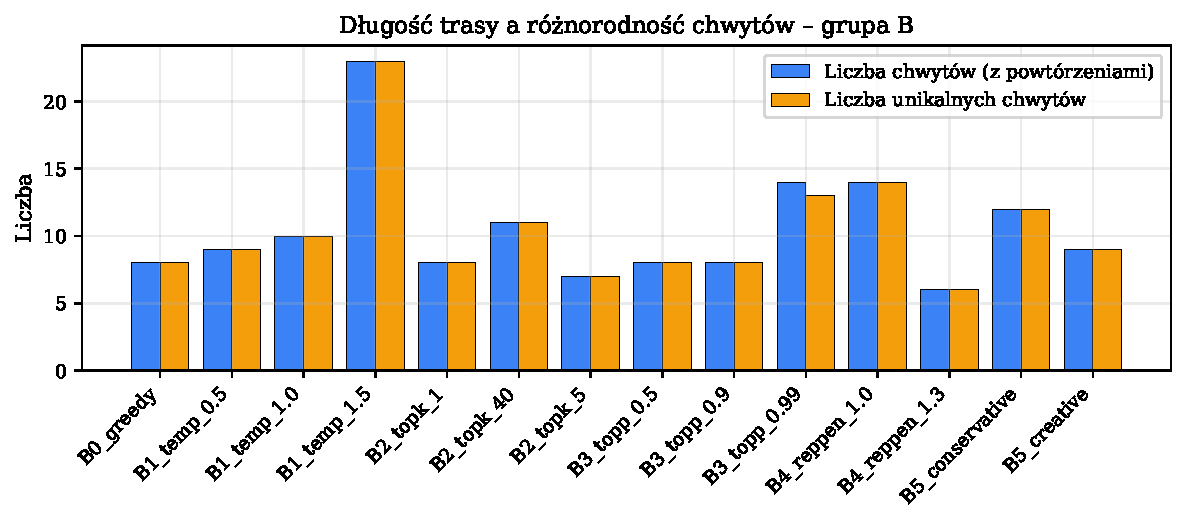
\includegraphics[width=0.97\linewidth]{fig_gen_lengths.pdf}
\caption{Liczba chwytów i liczba unikalnych chwytów w trasie wygenerowanej w każdym scenariuszu B.}
\label{fig:gen-lengths}
\end{figure}

\begin{figure}[H]
\centering
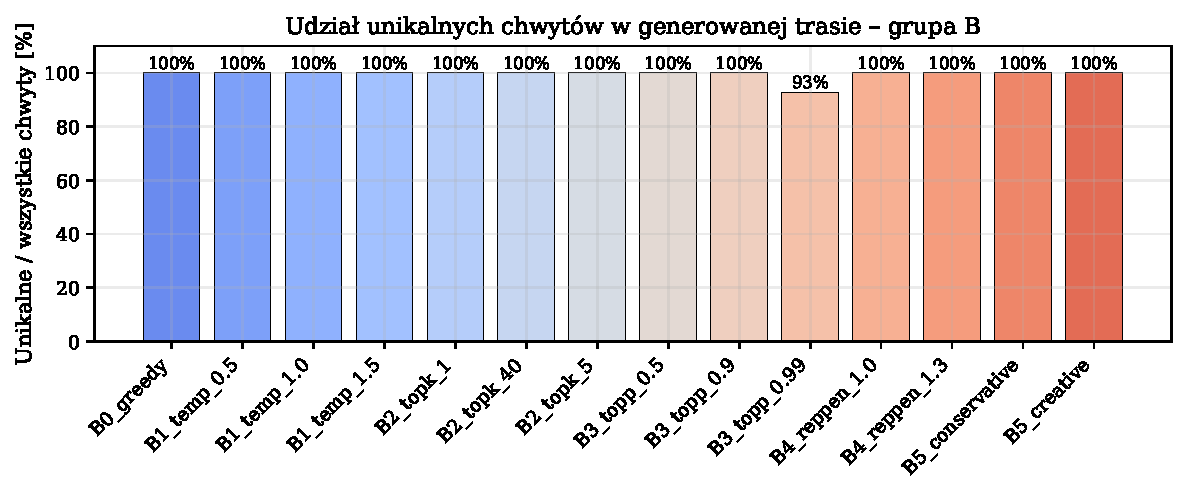
\includegraphics[width=0.97\linewidth]{fig_gen_unique_ratio.pdf}
\caption{Udział unikalnych chwytów w trasie. Wartość $<100\%$ świadczy o powtórzeniach.}
\label{fig:gen-unique}
\end{figure}

\paragraph{Temperatura $\tau$ (rys.~\ref{fig:gen-temp}).}
Wzrost $\tau$ z $0{,}5$ przez $1{,}0$ do $1{,}5$ wydłuża trasę z 9 do 10, a następnie do 23 chwytów. Trasa z $\tau=1{,}5$ traci jednak \emph{strukturę gramatyczną} (sekcja~\ref{sec:exp-quality}): pomiędzy tokenami \texttt{p1107}, \texttt{p1078}, \texttt{p1113}, \texttt{p1119}, \texttt{p1091} brakuje tokenów ról, a w generacji pojawia się rzadki rolowy token \texttt{r21}. To klasyczny przykład degeneracji wysokotemperaturowej \citep{holtzman2020nucleus}.

\begin{figure}[H]
\centering
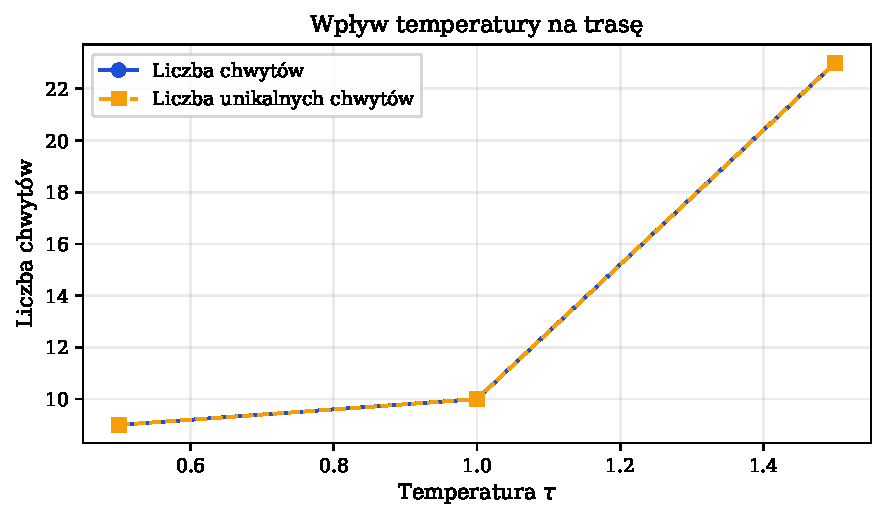
\includegraphics[width=0.7\linewidth]{fig_gen_temperature.pdf}
\caption{Wpływ temperatury $\tau$ na długość i różnorodność trasy.}
\label{fig:gen-temp}
\end{figure}

\paragraph{Top-$k$ (rys.~\ref{fig:gen-topk}).}
Dla $k=1$ próbkowanie redukuje się efektywnie do greedy --- ten sam wynik co B0 (8 chwytów). Bardzo małe $k=5$ skraca trasę do 7 chwytów, gdyż model bardzo szybko trafia na token \texttt{<EOS>}. Większe $k=40$ pozwala na 11 chwytów --- bliższe długości typowych tras V3 z korpusu.

\begin{figure}[H]
\centering
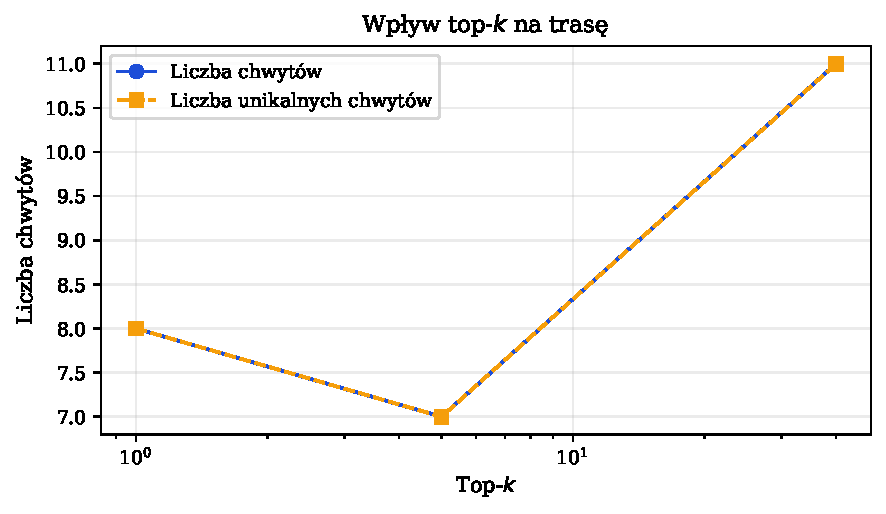
\includegraphics[width=0.7\linewidth]{fig_gen_topk.pdf}
\caption{Wpływ rozmiaru zbioru kandydatów top-$k$.}
\label{fig:gen-topk}
\end{figure}

\paragraph{Top-$p$ (rys.~\ref{fig:gen-topp}).}
Top-$p=0{,}5$ i $p=0{,}9$ generują w tym przypadku identycznie krótkie trasy ($n_h=8$). Dopiero $p=0{,}99$ dopuszcza wystarczająco szeroki ogon rozkładu, aby trasa wydłużyła się do 14 chwytów, lecz jednocześnie pojawia się powtórzenie chwytu \texttt{p1285} (ratio $13/14=92{,}9\%$). Ilustruje to kompromis \emph{coverage--quality}: zwiększanie $p$ zwiększa różnorodność, ale dopuszcza tokeny z mniej wiarygodnej części rozkładu.

\begin{figure}[H]
\centering
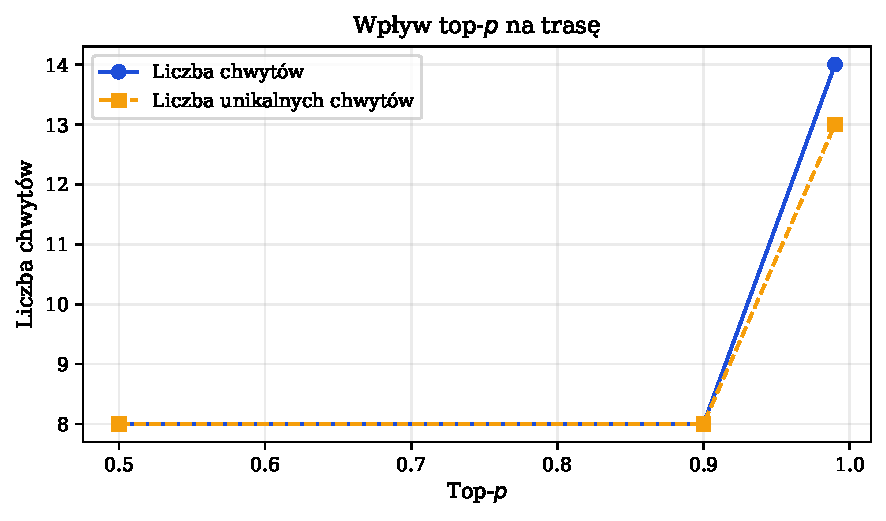
\includegraphics[width=0.7\linewidth]{fig_gen_topp.pdf}
\caption{Wpływ progu \emph{nucleus sampling} top-$p$.}
\label{fig:gen-topp}
\end{figure}

\paragraph{Repetition penalty $\rho$ (rys.~\ref{fig:gen-reppen}).}
Wyłączenie kary ($\rho=1{,}0$) prowadzi do trasy 14-chwytowej bez powtórzeń, co oznacza, że w tym scenariuszu dodatkowa penalizacja nie była konieczna. Wysoka wartość kary $\rho=1{,}3$ skraca trasę o ponad połowę (do 6 chwytów), gdyż token \texttt{<EOS>} uzyskuje relatywnie wyższe prawdopodobieństwo względem chwytów, które nie zostały jeszcze wykorzystane. Wskazuje to, że $\rho$ oddziałuje pośrednio także na długość generacji, nie tylko na samo unikanie powtórzeń.

\begin{figure}[H]
\centering
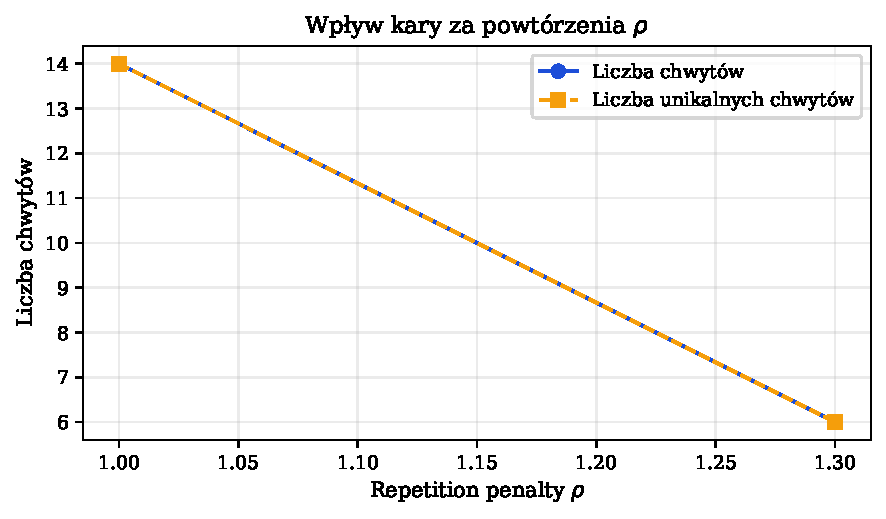
\includegraphics[width=0.7\linewidth]{fig_gen_reppen.pdf}
\caption{Wpływ kary za powtórzenia $\rho$.}
\label{fig:gen-reppen}
\end{figure}

\paragraph{Profil zachowawczy vs eksploracyjny.}
Konfiguracje B5 ilustrują wpływ jednoczesnej zmiany kilku parametrów dekodowania. \texttt{B5\_conservative} ($\tau=0{,}7$, $k=10$, $p=0{,}9$, $\rho=1{,}1$) generuje 12 chwytów --- długość zbliżoną do typowych tras V3 z korpusu. \texttt{B5\_creative} ($\tau=1{,}4$, $k=60$, $p=0{,}98$, $\rho=1{,}05$) generuje 9 mniej typowych chwytów; pojawia się mniej prawdopodobny token początkowy \texttt{p1157} w roli \texttt{r15} (start) zamiast częściej obserwowanych \texttt{p1107} / \texttt{p1181}.

\section{Analiza jakości i ograniczenia}
\label{sec:exp-quality}

\subsection{Mocne strony modelu}

Z analizy wygenerowanych tras wynika, że nawet stosunkowo prosty warunkowy dekoder GRU odwzorował trzy istotne cechy rozkładu:
\begin{enumerate}[leftmargin=1.5em]
    \item \textbf{Gramatyka przeplotu \texttt{p<id>}/\texttt{r<role>}.} W każdym scenariuszu B z umiarkowanymi parametrami ($\tau\le 1{,}0$, $p\le 0{,}9$) model generuje ścisłą sekwencję ,,chwyt --- rola --- chwyt --- rola...''. Taka gramatyka nie była wymuszona algorytmicznie, lecz wyłoniła się z danych.
    \item \textbf{Monotoniczne wznoszenie się.} Identyfikatory chwytów w wygenerowanych trasach niemal monotonicznie rosną wzdłuż sekwencji (np.\ B0\_greedy: \texttt{1154, 1181, 1219, 1235, 1285, 1304, 1353, 1390}). Numeracja otworów jest skorelowana z wysokością na panelu, więc model odtworzył fizyczny porządek ścieżki ,,od dołu do góry''.
    \item \textbf{Poprawne użycie ról.} Tokeny \texttt{r15} (start), \texttt{r12}/\texttt{r13} (chwyty pośrednie / na nogi), \texttt{r14} (top) pojawiają się we właściwych miejscach trasy --- \texttt{r14} zwykle blisko końca sekwencji.
\end{enumerate}

\subsection{Obserwowane błędy}

\paragraph{Degeneracja wysokotemperaturowa.}
W \texttt{B1\_temp\_1.5} model narusza gramatykę sekwencji (brak ról między czterema kolejnymi tokenami pozycji). Generuje także rzadko spotykany token \texttt{r21}, prawdopodobnie odpowiadający kategorii roli słabo reprezentowanej w korpusie.

\paragraph{Powtórzenia w ogonie rozkładu.}
W \texttt{B3\_topp\_0.99} pojawia się duplikat chwytu \texttt{p1285}. Bez aktywnej kary za powtórzenia ($\rho=1{,}0$) model sam korzysta z tej samej pozycji w sekwencji, mimo że w typowej trasie z korpusu chwyt nie wystąpi dwa razy.

\paragraph{Niestabilność uczenia przy zbyt dużym \texttt{lr}.}
W \texttt{A1\_lr\_high} (lr$=10^{-2}$) krzywe walidacji oscylują (epoki: $2{,}33 \to 2{,}23 \to 2{,}29 \to 2{,}23 \to 2{,}23$), zamiast monotonicznie maleć. Eksperymentalnie potwierdza to obserwację, że dla AdamW na zadaniach językowych $10^{-3}$ jest empirycznie korzystnym punktem pracy.

\paragraph{Sztuczne skracanie trasy przy dużym $\rho$.}
\texttt{B4\_reppen\_1.3} wskazuje, że wysoka kara za powtórzenia może wymusić przedwczesne pojawienie się \texttt{<EOS>} (trasa 6 chwytów zamiast typowych 8--12). Token \texttt{<EOS>} nie jest objęty karą, więc jego względne prawdopodobieństwo rośnie, gdy penalizowane są wszystkie wcześniej wygenerowane chwyty.

\subsection{Ograniczenia zastosowanej metodyki}

\begin{itemize}[leftmargin=1.5em]
    \item \textbf{Brak walidacji geometrycznej.} Model reprezentuje otwory wyłącznie jako abstrakcyjne tokeny i nie korzysta z ich współrzędnych (\textit{x}, \textit{y}) na panelu. Pozytywna obserwacja monotoniczności jest konsekwencją numerowania otworów, a nie eksplicytnego modelowania geometrii.
    \item \textbf{Brak kontroli długości.} Liczba chwytów w trasie jest pochodną parametrów dekodowania (zwłaszcza $\rho$ i $\tau$), nie zaś bezpośrednio sterowalnym warunkiem.
    \item \textbf{Pojedynczy holdout walidacyjny.} Pomiar \texttt{val\_nll} zależy od konkretnego splitu (sec.~\ref{sec:validation}). Stratyfikowana $k$-fold CV (np.\ po \texttt{grade\_id}) dałaby precyzyjniejszą estymację.
    \item \textbf{Ograniczony budżet treningowy w grupie A.} 5 epok na 20\,000 próbek służy jedynie przedstawieniu \emph{trendów}; bezwzględne wartości \texttt{best\_val\_nll} byłyby niższe przy 50 epokach na pełnym korpusie (porównaj \texttt{report\_full}: $0{,}858$).
    \item \textbf{Pojedynczy prompt w grupie B.} Wszystkie testy generacji wykonano na parze $(1272, 1240)$. Obserwacje dotyczące parametrów dekodowania pozostają jakościowo prawdziwe, ale konkretne długości tras $n_h$ należy traktować jako orientacyjne.
    \item \textbf{NLL jako wskaźnik zastępczy.} Niska wartość \texttt{val\_nll} nie jest jednoznaczna z wysoką jakością trasy z punktu widzenia wspinacza --- wymaga oceny eksperckiej lub dodatkowych metryk geometrycznych (długość kroków, rozproszenie chwytów).
\end{itemize}

\section{Wnioski}
\label{sec:conclusions}

\paragraph{Optymalna konfiguracja uczenia.}
Na podstawie tabeli~\ref{tab:exp-train} i krzywych z rysunków~\ref{fig:train-lr}--\ref{fig:summary-time} formułujemy następujący zestaw rekomendacji praktycznych dla zadania Kilter (zadanie modelowania krótkich sekwencji warunkowanych dwoma tokenami):
\begin{itemize}[leftmargin=1.5em]
    \item \textbf{Optymalizator}: AdamW z \texttt{lr}$=10^{-3}$, $\beta_1=0{,}9$, $\beta_2=0{,}999$. Niższe \texttt{lr} powoduje zauważalne niedouczenie, wyższe --- niestabilność.
    \item \textbf{Pojemność}: \texttt{embed\_dim}$=128$ i \texttt{hidden\_dim}$=256$ stanowią uzasadniony kompromis między jakością a kosztem. Przejście na model duży (\texttt{e}=256, \texttt{h}=512) jest uzasadnione dopiero przy odpowiednio większym budżecie obliczeniowym.
    \item \textbf{Liczba warstw GRU}: $1$--$3$. Pięć warstw nie poprawia wyników, a jednocześnie spowalnia zbieżność. Przy krótkich sekwencjach głębokie rekurencyjne dekodery są przeparametryzowane.
    \item \textbf{Dropout}: $0{,}0$--$0{,}15$ dla małych podzbiorów, $0{,}15$ dla pełnego korpusu. Dropout $0{,}5$ stanowi zbyt silną regularyzację.
    \item \textbf{Rozmiar batcha}: małe batche (16--64) działają lepiej niż duże (256). Mniejszy batch oznacza więcej kroków optymalizatora i bardziej stochastyczny gradient, co empirycznie poprawia generalizację na małym budżecie epok.
\end{itemize}

\paragraph{Optymalna konfiguracja dekodowania.}
Z grupy B wynika, że stabilnym domyślnym profilem do generacji użytecznych tras jest:
\begin{equation*}
\tau \in [0{,}7;\,1{,}0],\quad k \in [10;\,40],\quad p \in [0{,}9;\,0{,}95],\quad \rho \in [1{,}0;\,1{,}1].
\end{equation*}
Profile bardziej eksploracyjne (wyższe $\tau$, $k$, $p$) są dopuszczalne, ale wymagają postprocessingu odrzucającego wygenerowane trasy bez ról lub o nadmiernej długości.

\paragraph{Zachowania emergentne.}
Najistotniejszym jakościowym wnioskiem jest spontaniczne pojawienie się \emph{gramatyki przeplotu} chwyt/rola oraz porządku monotonicznego pozycji. Modele rekurencyjne z bardzo małą liczbą parametrów (\texttt{A2\_small}: $\sim 0{,}1$M parametrów) są w stanie uchwycić te regularności, co potwierdza, że indukcyjny bias GRU jest zgodny ze strukturą danych Kilter.

\paragraph{Limit obecnej architektury.}
Mimo poprawnej powierzchowej struktury, model nie uwzględnia jawnie \emph{geometrii panelu} ani \emph{biomechaniki ruchu}. Najczęstsze błędy generacji (degeneracja przy wysokim $\tau$, nieuzasadnione skracanie przy wysokim $\rho$) wskazują, że zwiększanie różnorodności wymaga uzupełnienia o moduł postprocesujący lub o jawne warunkowanie geometryczne.

\section{Dalsze kierunki rozwoju}
\label{sec:future-work}

\paragraph{Geometryczne warunkowanie modelu.}
Najistotniejszym kierunkiem jest dostarczenie modelowi informacji o pozycjach chwytów na panelu. Każdy otwór ma znaną parę współrzędnych $(x_i, y_i)$. Informację tę można uwzględnić przez:
\begin{itemize}[leftmargin=1.5em]
    \item statyczne wektory pozycyjne dodawane do \texttt{token\_embedding},
    \item wprowadzenie kontroli metrycznych odstępy między kolejnymi chwytami,
    \item warunkową funkcję kosztu karzącą fizycznie nierealne ruchy.
\end{itemize}

\paragraph{Architektury z mechanizmem uwagi.}
Zastąpienie GRU dekoderem typu Transformer \citep{sutskever2014seq2seq} z self-attention pozwoli modelować zależności pomiędzy odległymi chwytami bez kompresowania całej historii do jednego stanu ukrytego. Po wprowadzeniu \texttt{condition\_every\_step} kontekst $(\texttt{layout},\,\texttt{grade})$ jest już dostępny w każdym kroku GRU, jednak mechanizm uwagi nadal mógłby lepiej obsłużyć globalne zależności geometryczne i powtarzalne motywy ruchowe.

\paragraph{Zaawansowane strategie dekodowania.}
\begin{itemize}[leftmargin=1.5em]
    \item \emph{Beam search} z karą za długość --- alternatywa dla greedy gwarantująca stabilność.
    \item \emph{Contrastive decoding} --- generowanie z dwóch modeli (większego i mniejszego), zwiększające jakość.
    \item \emph{Reranker} --- generowanie $N$ kandydatów i wybór najlepszego według metryki geometrycznej.
\end{itemize}

\paragraph{Walidacja krzyżowa i hyperparameter search.}
W rozszerzonej fazie projektu warto zastosować:
\begin{itemize}[leftmargin=1.5em]
    \item stratyfikowaną $k$-fold CV po \texttt{grade\_id} (sekcja~\ref{sec:validation}),
    \item Bayesian/random search nad siatką \{\texttt{lr}, \texttt{hidden\_dim}, \texttt{layers}, \texttt{dropout}, \texttt{batch\_size}\} z biblioteką typu Optuna,
    \item early stopping z patience $=3$--$5$ oraz schedulerem typu \texttt{ReduceLROnPlateau}.
\end{itemize}

\paragraph{Sterowanie długością i stylem trasy.}
Wprowadzenie dodatkowych tokenów warunkujących, np.:
\begin{itemize}[leftmargin=1.5em]
    \item \texttt{<LEN=k>} --- pożądana liczba chwytów,
    \item \texttt{<STYLE=slab|overhang|dyno>} --- styl trasy,
\end{itemize}
pozwoli użytkownikowi dokładniej kontrolować generowany problem bez konieczności manipulowania parametrami dekodowania.

\paragraph{Ocena ekspercka.}
Pomiar \texttt{val\_nll} jest niezbędny, ale niewystarczający. Docelowo proponuje się zebranie pary ,,trasa wygenerowana / trasa eksperta'' i ocenę przez wspinaczy (np.\ w skali Likerta). To umożliwiłoby dostrojenie modelu metodą \emph{preference learning} (np.\ DPO), nawiązując do współczesnych technik RLHF stosowanych w modelach językowych.

\bibliography{raport}

\end{document}
